% Options for packages loaded elsewhere
% Options for packages loaded elsewhere
\PassOptionsToPackage{unicode}{hyperref}
\PassOptionsToPackage{hyphens}{url}
%
\documentclass[
  ignorenonframetext,
]{beamer}
\newif\ifbibliography
\usepackage{pgfpages}
\setbeamertemplate{caption}[numbered]
\setbeamertemplate{caption label separator}{: }
\setbeamercolor{caption name}{fg=normal text.fg}
\beamertemplatenavigationsymbolsempty
% remove section numbering
\setbeamertemplate{part page}{
  \centering
  \begin{beamercolorbox}[sep=16pt,center]{part title}
    \usebeamerfont{part title}\insertpart\par
  \end{beamercolorbox}
}
\setbeamertemplate{section page}{
  \centering
  \begin{beamercolorbox}[sep=12pt,center]{section title}
    \usebeamerfont{section title}\insertsection\par
  \end{beamercolorbox}
}
\setbeamertemplate{subsection page}{
  \centering
  \begin{beamercolorbox}[sep=8pt,center]{subsection title}
    \usebeamerfont{subsection title}\insertsubsection\par
  \end{beamercolorbox}
}
% Prevent slide breaks in the middle of a paragraph
\widowpenalties 1 10000
\raggedbottom
\AtBeginPart{
  \frame{\partpage}
}
\AtBeginSection{
  \ifbibliography
  \else
    \frame{\sectionpage}
  \fi
}
\AtBeginSubsection{
  \frame{\subsectionpage}
}
\usepackage{iftex}
\ifPDFTeX
  \usepackage[T1]{fontenc}
  \usepackage[utf8]{inputenc}
  \usepackage{textcomp} % provide euro and other symbols
\else % if luatex or xetex
  \usepackage{unicode-math} % this also loads fontspec
  \defaultfontfeatures{Scale=MatchLowercase}
  \defaultfontfeatures[\rmfamily]{Ligatures=TeX,Scale=1}
\fi
\usepackage{lmodern}

\usetheme[]{Madrid}
\usecolortheme[]{dolphin}
\ifPDFTeX\else
  % xetex/luatex font selection
\fi
% Use upquote if available, for straight quotes in verbatim environments
\IfFileExists{upquote.sty}{\usepackage{upquote}}{}
\IfFileExists{microtype.sty}{% use microtype if available
  \usepackage[]{microtype}
  \UseMicrotypeSet[protrusion]{basicmath} % disable protrusion for tt fonts
}{}
\makeatletter
\@ifundefined{KOMAClassName}{% if non-KOMA class
  \IfFileExists{parskip.sty}{%
    \usepackage{parskip}
  }{% else
    \setlength{\parindent}{0pt}
    \setlength{\parskip}{6pt plus 2pt minus 1pt}}
}{% if KOMA class
  \KOMAoptions{parskip=half}}
\makeatother

\usepackage{color}
\usepackage{fancyvrb}
\newcommand{\VerbBar}{|}
\newcommand{\VERB}{\Verb[commandchars=\\\{\}]}
\DefineVerbatimEnvironment{Highlighting}{Verbatim}{commandchars=\\\{\}}
% Add ',fontsize=\small' for more characters per line
\usepackage{framed}
\definecolor{shadecolor}{RGB}{241,243,245}
\newenvironment{Shaded}{\begin{snugshade}}{\end{snugshade}}
\newcommand{\AlertTok}[1]{\textcolor[rgb]{0.68,0.00,0.00}{#1}}
\newcommand{\AnnotationTok}[1]{\textcolor[rgb]{0.37,0.37,0.37}{#1}}
\newcommand{\AttributeTok}[1]{\textcolor[rgb]{0.40,0.45,0.13}{#1}}
\newcommand{\BaseNTok}[1]{\textcolor[rgb]{0.68,0.00,0.00}{#1}}
\newcommand{\BuiltInTok}[1]{\textcolor[rgb]{0.00,0.23,0.31}{#1}}
\newcommand{\CharTok}[1]{\textcolor[rgb]{0.13,0.47,0.30}{#1}}
\newcommand{\CommentTok}[1]{\textcolor[rgb]{0.37,0.37,0.37}{#1}}
\newcommand{\CommentVarTok}[1]{\textcolor[rgb]{0.37,0.37,0.37}{\textit{#1}}}
\newcommand{\ConstantTok}[1]{\textcolor[rgb]{0.56,0.35,0.01}{#1}}
\newcommand{\ControlFlowTok}[1]{\textcolor[rgb]{0.00,0.23,0.31}{\textbf{#1}}}
\newcommand{\DataTypeTok}[1]{\textcolor[rgb]{0.68,0.00,0.00}{#1}}
\newcommand{\DecValTok}[1]{\textcolor[rgb]{0.68,0.00,0.00}{#1}}
\newcommand{\DocumentationTok}[1]{\textcolor[rgb]{0.37,0.37,0.37}{\textit{#1}}}
\newcommand{\ErrorTok}[1]{\textcolor[rgb]{0.68,0.00,0.00}{#1}}
\newcommand{\ExtensionTok}[1]{\textcolor[rgb]{0.00,0.23,0.31}{#1}}
\newcommand{\FloatTok}[1]{\textcolor[rgb]{0.68,0.00,0.00}{#1}}
\newcommand{\FunctionTok}[1]{\textcolor[rgb]{0.28,0.35,0.67}{#1}}
\newcommand{\ImportTok}[1]{\textcolor[rgb]{0.00,0.46,0.62}{#1}}
\newcommand{\InformationTok}[1]{\textcolor[rgb]{0.37,0.37,0.37}{#1}}
\newcommand{\KeywordTok}[1]{\textcolor[rgb]{0.00,0.23,0.31}{\textbf{#1}}}
\newcommand{\NormalTok}[1]{\textcolor[rgb]{0.00,0.23,0.31}{#1}}
\newcommand{\OperatorTok}[1]{\textcolor[rgb]{0.37,0.37,0.37}{#1}}
\newcommand{\OtherTok}[1]{\textcolor[rgb]{0.00,0.23,0.31}{#1}}
\newcommand{\PreprocessorTok}[1]{\textcolor[rgb]{0.68,0.00,0.00}{#1}}
\newcommand{\RegionMarkerTok}[1]{\textcolor[rgb]{0.00,0.23,0.31}{#1}}
\newcommand{\SpecialCharTok}[1]{\textcolor[rgb]{0.37,0.37,0.37}{#1}}
\newcommand{\SpecialStringTok}[1]{\textcolor[rgb]{0.13,0.47,0.30}{#1}}
\newcommand{\StringTok}[1]{\textcolor[rgb]{0.13,0.47,0.30}{#1}}
\newcommand{\VariableTok}[1]{\textcolor[rgb]{0.07,0.07,0.07}{#1}}
\newcommand{\VerbatimStringTok}[1]{\textcolor[rgb]{0.13,0.47,0.30}{#1}}
\newcommand{\WarningTok}[1]{\textcolor[rgb]{0.37,0.37,0.37}{\textit{#1}}}

\usepackage{longtable,booktabs,array}
\usepackage{calc} % for calculating minipage widths
\usepackage{caption}
% Make caption package work with longtable
\makeatletter
\def\fnum@table{\tablename~\thetable}
\makeatother
\usepackage{graphicx}
\makeatletter
\newsavebox\pandoc@box
\newcommand*\pandocbounded[1]{% scales image to fit in text height/width
  \sbox\pandoc@box{#1}%
  \Gscale@div\@tempa{\textheight}{\dimexpr\ht\pandoc@box+\dp\pandoc@box\relax}%
  \Gscale@div\@tempb{\linewidth}{\wd\pandoc@box}%
  \ifdim\@tempb\p@<\@tempa\p@\let\@tempa\@tempb\fi% select the smaller of both
  \ifdim\@tempa\p@<\p@\scalebox{\@tempa}{\usebox\pandoc@box}%
  \else\usebox{\pandoc@box}%
  \fi%
}
% Set default figure placement to htbp
\def\fps@figure{htbp}
\makeatother





\setlength{\emergencystretch}{3em} % prevent overfull lines

\providecommand{\tightlist}{%
  \setlength{\itemsep}{0pt}\setlength{\parskip}{0pt}}



 


\makeatletter
\@ifpackageloaded{caption}{}{\usepackage{caption}}
\AtBeginDocument{%
\ifdefined\contentsname
  \renewcommand*\contentsname{Table of contents}
\else
  \newcommand\contentsname{Table of contents}
\fi
\ifdefined\listfigurename
  \renewcommand*\listfigurename{List of Figures}
\else
  \newcommand\listfigurename{List of Figures}
\fi
\ifdefined\listtablename
  \renewcommand*\listtablename{List of Tables}
\else
  \newcommand\listtablename{List of Tables}
\fi
\ifdefined\figurename
  \renewcommand*\figurename{Figure}
\else
  \newcommand\figurename{Figure}
\fi
\ifdefined\tablename
  \renewcommand*\tablename{Table}
\else
  \newcommand\tablename{Table}
\fi
}
\@ifpackageloaded{float}{}{\usepackage{float}}
\floatstyle{ruled}
\@ifundefined{c@chapter}{\newfloat{codelisting}{h}{lop}}{\newfloat{codelisting}{h}{lop}[chapter]}
\floatname{codelisting}{Listing}
\newcommand*\listoflistings{\listof{codelisting}{List of Listings}}
\makeatother
\makeatletter
\makeatother
\makeatletter
\@ifpackageloaded{caption}{}{\usepackage{caption}}
\@ifpackageloaded{subcaption}{}{\usepackage{subcaption}}
\makeatother

\usepackage{bookmark}
\IfFileExists{xurl.sty}{\usepackage{xurl}}{} % add URL line breaks if available
\urlstyle{same}
\hypersetup{
  pdftitle={Redes LSTM: Memoria a Largo y Corto Plazo},
  pdfauthor={Presentación sobre Redes Neuronales Recurrentes},
  hidelinks,
  pdfcreator={LaTeX via pandoc}}


\title{Redes LSTM: Memoria a Largo y Corto Plazo}
\subtitle{Arquitectura y Funcionamiento Detallado}
\author{Presentación sobre Redes Neuronales Recurrentes}
\date{2025-10-01}

\begin{document}
\frame{\titlepage}


\begin{frame}{¿Qué son las LSTM?}
\phantomsection\label{quuxe9-son-las-lstm}
\begin{itemize}
\tightlist
\item
  \textbf{Extensión de las RNN} diseñadas para capturar dependencias
  temporales de secuencias largas
\item
  Las RNN básicas \textbf{luchan por capturar} dependencias largas en el
  tiempo
\item
  Introducen el concepto de \textbf{``celda de memoria''} que puede
  mantener, escribir o leer información
\item
  Controladas por \textbf{estructuras llamadas puertas} que gestionan el
  flujo de información
\end{itemize}
\end{frame}

\begin{frame}{Problemas que Resuelven las LSTM}
\phantomsection\label{problemas-que-resuelven-las-lstm}
\begin{block}{Limitaciones de las RNN Básicas}
\phantomsection\label{limitaciones-de-las-rnn-buxe1sicas}
\begin{itemize}
\tightlist
\item
  \textbf{Problema del gradiente de fuga}
\item
  Dificultad para considerar \textbf{secuencias de entrada largas}
\item
  \textbf{Pérdida de contexto} en dependencias temporales largas
\end{itemize}
\end{block}

\begin{block}{Soluciones de las LSTM}
\phantomsection\label{soluciones-de-las-lstm}
\begin{itemize}
\tightlist
\item
  Las alteraciones en los LSTM \textbf{abordan el problema del gradiente
  de fuga}
\item
  Permiten considerar \textbf{secuencias de entrada mucho más largas}
\item
  \textbf{Preservan el contexto} de manera más efectiva
\end{itemize}
\end{block}
\end{frame}

\begin{frame}{Arquitectura LSTM: Las Tres Puertas}
\phantomsection\label{arquitectura-lstm-las-tres-puertas}
\begin{block}{Componentes Fundamentales}
\phantomsection\label{componentes-fundamentales}
\begin{enumerate}
\tightlist
\item
  \textbf{Puerta de entrada} - Decide qué valores son importantes
\item
  \textbf{Puerta de olvido} - Descarta información innecesaria\\
\item
  \textbf{Puerta de salida} - Decide qué información pasar al siguiente
  paso
\end{enumerate}
\end{block}

\begin{block}{Características Comunes}
\phantomsection\label{caracteruxedsticas-comunes}
\begin{itemize}
\tightlist
\item
  Consideran las \textbf{entradas del paso de tiempo anterior}
\item
  Modifican la \textbf{memoria del modelo} y los \textbf{pesos de
  entrada}
\item
  Utilizan \textbf{funciones de activación específicas} para cada puerta
\end{itemize}

\begin{figure}[H]

{\centering 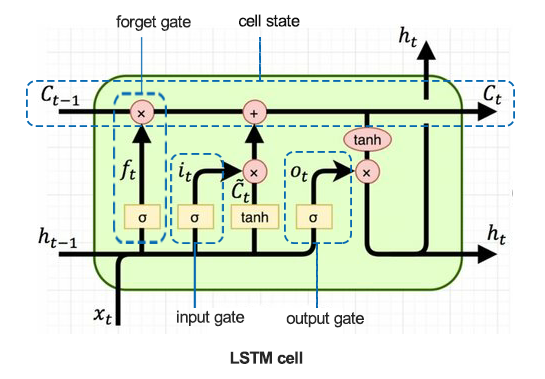
\includegraphics[width=0.5\linewidth,height=\textheight,keepaspectratio]{LSTM.png}

}

\caption{Arquitectura LSTM}

\end{figure}%
\end{block}
\end{frame}

\begin{frame}{Puerta de Olvido}
\phantomsection\label{puerta-de-olvido}
\begin{block}{Función Principal}
\phantomsection\label{funciuxf3n-principal}
Descarta \textbf{información que el modelo considera innecesaria} para
tomar decisiones. Ecuación Matemática
\[f_t = \sigma(W_f \cdot [h_{t-1}, x_t] + b_f)\]
\end{block}

\begin{block}{Componentes}
\phantomsection\label{componentes}
\begin{itemize}
\tightlist
\item
  \(W_f\): \textbf{peso de la puerta del olvido}
\item
  \(b_f\): \textbf{sesgo de la puerta de olvido}
\item
  \(\sigma\): \textbf{función sigmoidea} (valores 0-1)
\end{itemize}
\end{block}

\begin{block}{Interpretación}
\phantomsection\label{interpretaciuxf3n}
\begin{itemize}
\tightlist
\item
  \textbf{0}: Olvidar completamente
\item
  \textbf{1}: Retener completamente
\item
  Determina qué información del estado anterior conservar
\end{itemize}
\end{block}
\end{frame}

\begin{frame}{Puerta de Entrada}
\phantomsection\label{puerta-de-entrada}
\begin{block}{Función Principal}
\phantomsection\label{funciuxf3n-principal-1}
Decide \textbf{qué valores son importantes} y deben transmitirse por el
modelo.
\end{block}

\begin{block}{Ecuaciones}
\phantomsection\label{ecuaciones}
\textbf{Decidir qué actualizar:}
\[i_t = \sigma(W_i \cdot [h_{t-1}, x_t] + b_i)\]

\textbf{Generar valores candidatos:}
\[\tilde{C}_t = \tanh(W_C \cdot [h_{t-1}, x_t] + b_C)\]
\end{block}

\begin{block}{Funciones de Activación}
\phantomsection\label{funciones-de-activaciuxf3n}
\begin{itemize}
\tightlist
\item
  \textbf{Sigmoidea}: decide qué valores transmitir (0 = reducir, 1 =
  conservar)
\item
  \textbf{TanH}: decide importancia de valores (-1 a 1)
\end{itemize}
\end{block}
\end{frame}

\begin{frame}{Célula de Memoria Candidata}
\phantomsection\label{cuxe9lula-de-memoria-candidata}
\begin{block}{Función}
\phantomsection\label{funciuxf3n}
Genera \textbf{nueva información potencial} para almacenar en el estado
de la celda.
\end{block}

\begin{block}{Ecuación}
\phantomsection\label{ecuaciuxf3n}
\[\tilde{C}_t = \tanh(W_C \cdot [h_{t-1}, x_t] + b_C)\]
\end{block}

\begin{block}{Características}
\phantomsection\label{caracteruxedsticas}
\begin{itemize}
\tightlist
\item
  Genera \textbf{valores candidatos} para agregar al estado
\item
  Función \textbf{tanh} asegura valores entre -1 y 1
\item
  Representa \textbf{información potencial} para almacenar
\end{itemize}
\end{block}
\end{frame}

\begin{frame}{Actualización del Estado de la Celda}
\phantomsection\label{actualizaciuxf3n-del-estado-de-la-celda}
\begin{block}{Proceso de Actualización}
\phantomsection\label{proceso-de-actualizaciuxf3n}
\[C_t = f_t \cdot C_{t-1} + i_t \cdot \tilde{C}_t\]
\end{block}

\begin{block}{Explicación del Proceso}
\phantomsection\label{explicaciuxf3n-del-proceso}
\begin{enumerate}
\tightlist
\item
  Estado anterior (\(C_{t-1}\)) × Puerta de olvido (\(f_t\))
\item
  Valores candidatos (\(\tilde{C}_t\)) × Puerta de entrada (\(i_t\))
\item
  \textbf{Suma} para formar nuevo estado (\(C_t\))
\end{enumerate}
\end{block}

\begin{block}{Interpretación}
\phantomsection\label{interpretaciuxf3n-1}
Combina información conservada con nueva información importante.
\end{block}
\end{frame}

\begin{frame}{Puerta de Salida}
\phantomsection\label{puerta-de-salida}
\begin{block}{Función Principal}
\phantomsection\label{funciuxf3n-principal-2}
Decide \textbf{qué valores pasar al siguiente paso de tiempo}.
\end{block}

\begin{block}{Ecuación}
\phantomsection\label{ecuaciuxf3n-1}
\[o_t = \sigma(W_o \cdot [h_{t-1}, x_t] + b_o)\]
\end{block}

\begin{block}{Proceso de Decisión}
\phantomsection\label{proceso-de-decisiuxf3n}
\begin{itemize}
\tightlist
\item
  Analiza valores y asigna importancia (-1 a 1)
\item
  Regula datos antes del siguiente cálculo
\item
  Decide \textbf{salida final} del estado actual
\end{itemize}
\end{block}
\end{frame}

\begin{frame}{Actualización del Estado Oculto}
\phantomsection\label{actualizaciuxf3n-del-estado-oculto}
\begin{block}{Ecuación Final}
\phantomsection\label{ecuaciuxf3n-final}
\[h_t = o_t \cdot \tanh(C_t)\]
\end{block}

\begin{block}{Funcionalidad}
\phantomsection\label{funcionalidad}
\begin{itemize}
\tightlist
\item
  Estado oculto se actualiza según estado de celda y puerta de salida
\item
  Se usa como \textbf{salida para paso actual}
\item
  Sirve como \textbf{entrada para siguiente paso}
\end{itemize}
\end{block}
\end{frame}

\begin{frame}{Flujo Completo LSTM}
\phantomsection\label{flujo-completo-lstm}
\begin{block}{Proceso Secuencial}
\phantomsection\label{proceso-secuencial}
\begin{enumerate}
\tightlist
\item
  \textbf{Puerta de Olvido}: Qué información conservar (sigmoidea 0-1)
\item
  \textbf{Puerta de Entrada}: Qué nueva información incorporar
  (sigmoidea + tanh)
\item
  \textbf{Actualización Estado}:
  \(C_t = f_t \cdot C_{t-1} + i_t \cdot \tilde{C}_t\)
\item
  \textbf{Puerta de Salida}: Qué información emitir (sigmoidea)
\item
  \textbf{Estado Oculto}: \(h_t = o_t \cdot \tanh(C_t)\)
\end{enumerate}
\end{block}
\end{frame}

\begin{frame}{Aplicaciones Prácticas}
\phantomsection\label{aplicaciones-pruxe1cticas}
\begin{block}{Campos de Uso}
\phantomsection\label{campos-de-uso}
\begin{itemize}
\tightlist
\item
  \textbf{Procesamiento de lenguaje natural}
\item
  \textbf{Reconocimiento de voz}
\item
  \textbf{Predicción de series temporales}
\item
  \textbf{Sistemas de recomendación}
\item
  \textbf{Análisis de datos secuenciales}
\end{itemize}
\end{block}

\begin{block}{Beneficios Clave}
\phantomsection\label{beneficios-clave}
\begin{itemize}
\tightlist
\item
  \textbf{Manejan dependencias largas} eficientemente
\item
  \textbf{Resuelven problema del gradiente de fuga}
\item
  \textbf{Preservan contexto} en secuencias largas
\item
  \textbf{Flexibles} para diversos datos temporales
\end{itemize}
\end{block}

\begin{block}{Impacto}
\phantomsection\label{impacto}
Las LSTM representan \textbf{evolución significativa} sobre RNN
tradicionales, permitiendo manejo efectivo de \textbf{dependencias
temporales largas}.
\end{block}
\end{frame}

\begin{frame}{¿Qué es una capa LSTM en el contexto de inundaciones?}
\phantomsection\label{quuxe9-es-una-capa-lstm-en-el-contexto-de-inundaciones}
Es una capa de red neuronal recurrente especializada en procesar
\textbf{datos secuenciales temporales}:

\begin{itemize}
\tightlist
\item
  Series de tiempo de \textbf{niveles de ríos}
\item
  Datos de \textbf{precipitación} acumulada\\
\item
  \textbf{Humedad del suelo} histórica
\item
  Variables meteorológicas temporales
\end{itemize}

\textbf{Diseño con ``puertas''} le permite: - Recordar \textbf{patrones
importantes} (picos de lluvia antecedentes) - Olvidar
\textbf{información irrelevante} (días sin lluvia) - Predecir
\textbf{eventos extremos} con horas/días de anticipación
\end{frame}

\begin{frame}{Parámetros principales (en contexto de inundaciones)}
\phantomsection\label{paruxe1metros-principales-en-contexto-de-inundaciones}
\begin{block}{Configuración clave para hidrología}
\phantomsection\label{configuraciuxf3n-clave-para-hidrologuxeda}
\textbf{units} → Número de celdas LSTM. Más unidades capturan patrones
complejos\\
\emph{Ejemplo: 50 unidades para predecir crecidas en una cuenca grande}

\textbf{return\_sequences} → Si es True, devuelve salidas en cada paso
temporal\\
\emph{Útil para conectar otra LSTM después}

\textbf{return\_state} → Devuelve estados internos\\
\emph{Para modelos avanzados de atención o inicialización}

\textbf{activation} → Función de activación\\
\emph{Por defecto tanh para estabilidad}

\textbf{input\_shape} → Forma de la entrada: (pasos\_temporales,
características)\\
\emph{Ejemplo: (30, 5) para 30 días con 5 variables meteorológicas}
\end{block}
\end{frame}

\begin{frame}{Ejemplo conceptual con datos reales}
\phantomsection\label{ejemplo-conceptual-con-datos-reales}
\begin{block}{Secuencia de 7 días de datos hidrológicos}
\phantomsection\label{secuencia-de-7-duxedas-de-datos-hidroluxf3gicos}
\textbf{Entrada (7 días × 4 características):}

\begin{longtable}[]{@{}lllll@{}}
\toprule\noalign{}
Día & Precipitación & Nivel Río & Humedad Suelo & Temperatura \\
\midrule\noalign{}
\endhead
1 & 5mm & 2.0m & 60\% & 20°C \\
2 & 10mm & 2.2m & 70\% & 18°C \\
3 & 25mm & 2.5m & 80\% & 16°C \\
4 & 40mm & 2.8m & 85\% & 15°C \\
5 & 35mm & 3.0m & 90\% & 14°C \\
6 & 45mm & 3.2m & 92\% & 15°C \\
7 & 50mm & 3.5m & 95\% & 15°C \\
\bottomrule\noalign{}
\end{longtable}
\end{block}

\begin{block}{Procesamiento LSTM}
\phantomsection\label{procesamiento-lstm}
Una LSTM con \textbf{units=3} procesará esta secuencia día a día,
actualizando su \textbf{``memoria''} con la evolución de las variables.
\end{block}
\end{frame}

\begin{frame}[fragile]{Ejemplo interpretativo para predicción de
inundaciones}
\phantomsection\label{ejemplo-interpretativo-para-predicciuxf3n-de-inundaciones}
\begin{block}{Configuración del modelo}
\phantomsection\label{configuraciuxf3n-del-modelo}
\texttt{LSTM(units=10,\ return\_sequences=False,\ input\_shape=(30,\ 6))}

\begin{block}{a) Entrada}
\phantomsection\label{a-entrada}
30 días históricos con 6 variables: - Precipitación - Nivel del río\\
- Humedad del suelo - Temperatura - Velocidad del viento - Presión
atmosférica
\end{block}

\begin{block}{b) Proceso}
\phantomsection\label{b-proceso}
\textbf{units=10} → La capa tiene 10 celdas LSTM para capturar patrones
complejos\\
\emph{Ejemplo: correlaciones entre lluvia acumulada y subida del río}

\textbf{return\_sequences=False} → Solo devuelve la salida del último
día\\
\emph{Para predecir inundación al día siguiente}

\textbf{Puertas de olvido} descartan datos no relevantes\\
\emph{Ejemplo: días secos antiguos}

\textbf{Puertas de entrada} guardan información crítica\\
\emph{Ejemplo: lluvia intensa reciente}
\end{block}

\begin{block}{c) Salida}
\phantomsection\label{c-salida}
\textbf{Forma}: (batch\_size, 10)

\textbf{Interpretación}: Cada valor del vector representa un patrón
aprendido: - Valor 1: ``alta humedad acumulada'' - Valor 2: ``tendencia
de subida rápida del río'' - Valor 3: ``patrón de precipitación
intensa'' - \ldots{} etc.

Este vector se alimenta a una capa densa para predecir
\textbf{probabilidad de inundación}.
\end{block}
\end{block}
\end{frame}

\begin{frame}{Analogía intuitiva}
\phantomsection\label{analoguxeda-intuitiva}
Piensa en la LSTM como un \textbf{experto en hidrología} que analiza un
informe diario:

Forget gate

Como cuando decide que una \textbf{lluvia leve de hace 20 días} ya no es
relevante para el riesgo actual.

Input gate\\
Cuando subraya datos importantes: \textbf{``¡Lluvia de 100mm en 3
días!''}

Output gate Cuando emite un alerta gradual: \textbf{``Río subiendo
0.5m/día → riesgo en 48h''}

Evolución del análisis

\begin{itemize}
\item
  \textbf{Capas simples}: Variables individuales
\item
  \textbf{Capas múltiples}: Interacciones complejas
\item
  \textbf{Ejemplo avanzado}: ``Suelo saturado + lluvia intensa =
  inundación repentina''
\end{itemize}
\end{frame}

\begin{frame}{Mini-ejemplo numérico simplificado}
\phantomsection\label{mini-ejemplo-numuxe9rico-simplificado}
\begin{block}{Entrada de 3 días para predecir crecida}
\phantomsection\label{entrada-de-3-duxedas-para-predecir-crecida}
\begin{longtable}[]{@{}llll@{}}
\toprule\noalign{}
Día & Precipitación & Nivel Río & Normalizado \\
\midrule\noalign{}
\endhead
1 & 10mm & 1.5m & {[}0.1, 0.15{]} \\
2 & 30mm & 1.7m & {[}0.3, 0.17{]} \\
3 & 60mm & 2.0m & {[}0.6, 0.2{]} \\
\bottomrule\noalign{}
\end{longtable}
\end{block}

\begin{block}{Procesamiento paso a paso}
\phantomsection\label{procesamiento-paso-a-paso}
\textbf{Estado inicial}: h₀ = {[}0, 0{]}, c₀ = {[}0, 0{]}

\textbf{Paso 1 (Día 1)}: - LSTM detecta lluvia moderada → actualiza
ligeramente su estado - h₁ = {[}0.02, 0.01{]}, c₁ = {[}0.03, 0.02{]}

\textbf{Paso 2 (Día 2)}: - Lluvia alta → puerta de entrada guarda esta
información - h₂ = {[}0.15, 0.1{]}, c₂ = {[}0.2, 0.12{]}

\textbf{Paso 3 (Día 3)}: - Lluvia extrema + nivel subiendo → puerta de
olvido mantiene todo el historial reciente - \textbf{Salida}: h₃ =
{[}0.8, 0.6{]} (indica alto riesgo)
\end{block}

\begin{block}{Resultado final}
\phantomsection\label{resultado-final}
Una capa densa traduce esto a: \textbf{Probabilidad\_inundación = 85\%}
\end{block}
\end{frame}

\begin{frame}{¿Por qué es útil para inundaciones?}
\phantomsection\label{por-quuxe9-es-uxfatil-para-inundaciones}
\begin{block}{Captura la no linealidad de las cuencas}
\phantomsection\label{captura-la-no-linealidad-de-las-cuencas}
\emph{Ejemplo: el suelo se satura después de X días de lluvia}
\end{block}

\begin{block}{Modela retrasos temporales}
\phantomsection\label{modela-retrasos-temporales}
\emph{Ejemplo: la lluvia tarda horas en afectar el río aguas abajo}
\end{block}

\begin{block}{Puede integrar múltiples fuentes de datos}
\phantomsection\label{puede-integrar-muxfaltiples-fuentes-de-datos}
\begin{itemize}
\tightlist
\item
  Satélites
\item
  Sensores terrestres\\
\item
  Pronósticos meteorológicos
\end{itemize}
\end{block}

\begin{block}{Usada en sistemas de alerta temprana}
\phantomsection\label{usada-en-sistemas-de-alerta-temprana}
Como el \textbf{EFAS} (European Flood Awareness System)
\end{block}
\end{frame}

\begin{frame}{Resumen de ventajas}
\phantomsection\label{resumen-de-ventajas}
\begin{block}{Para predicción hidrológica}
\phantomsection\label{para-predicciuxf3n-hidroluxf3gica}
\begin{itemize}
\tightlist
\item
  \textbf{Memoria persistente} para eventos lejanos críticos
\item
  \textbf{Adaptabilidad} a diferentes tipos de cuencas
\item
  \textbf{Robustez} con datos imperfectos o incompletos
\end{itemize}
\end{block}

\begin{block}{Para gestión de emergencias}
\phantomsection\label{para-gestiuxf3n-de-emergencias}
\begin{itemize}
\tightlist
\item
  \textbf{Alertas tempranas} con mayor anticipación
\item
  \textbf{Mejor precisión} en predicción de eventos extremos
\item
  \textbf{Integración} de múltiples fuentes de información
\end{itemize}
\end{block}
\end{frame}

\begin{frame}{Aplicaciones en sistemas reales}
\phantomsection\label{aplicaciones-en-sistemas-reales}
\begin{block}{Casos de implementación}
\phantomsection\label{casos-de-implementaciuxf3n}
\begin{itemize}
\tightlist
\item
  \textbf{Sistemas de alerta temprana} nacionales y regionales
\item
  \textbf{Monitoreo de cuencas} críticas
\item
  \textbf{Predicción de crecidas} repentinas
\item
  \textbf{Gestión de embalses} y recursos hídricos
\end{itemize}
\end{block}

\begin{block}{Beneficios demostrados}
\phantomsection\label{beneficios-demostrados}
\begin{itemize}
\tightlist
\item
  \textbf{Reducción de daños} económicos
\item
  \textbf{Protección de vidas} humanas
\item
  \textbf{Optimización} de recursos de emergencia
\item
  \textbf{Mejora} en la toma de decisiones
\end{itemize}
\end{block}
\end{frame}

\begin{frame}[fragile]{Generación de Datos de Inundaciones}
\phantomsection\label{generaciuxf3n-de-datos-de-inundaciones}
\phantomsection\label{gen-datos}
\begin{Shaded}
\begin{Highlighting}[]
\CommentTok{\# =============================}
\CommentTok{\# 1. IMPORTAR LIBRERÍAS Y GENERAR DATOS DE INUNDACIONES}
\CommentTok{\# ===============================}
\ImportTok{import}\NormalTok{ numpy }\ImportTok{as}\NormalTok{ np}
\ImportTok{import}\NormalTok{ pandas }\ImportTok{as}\NormalTok{ pd}
\ImportTok{import}\NormalTok{ matplotlib.pyplot }\ImportTok{as}\NormalTok{ plt}
\ImportTok{import}\NormalTok{ tensorflow }\ImportTok{as}\NormalTok{ tf}
\ImportTok{from}\NormalTok{ tensorflow.keras.models }\ImportTok{import}\NormalTok{ Sequential}
\ImportTok{from}\NormalTok{ tensorflow.keras.layers }\ImportTok{import}\NormalTok{ LSTM, Dense, Dropout, Input}
\ImportTok{from}\NormalTok{ tensorflow.keras.optimizers }\ImportTok{import}\NormalTok{ Adam}
\ImportTok{from}\NormalTok{ tensorflow.keras.callbacks }\ImportTok{import}\NormalTok{ EarlyStopping}
\ImportTok{from}\NormalTok{ sklearn.preprocessing }\ImportTok{import}\NormalTok{ MinMaxScaler}
\ImportTok{from}\NormalTok{ sklearn.metrics }\ImportTok{import}\NormalTok{ accuracy\_score, classification\_report, confusion\_matrix}
\ImportTok{from}\NormalTok{ tensorflow.keras.metrics }\ImportTok{import}\NormalTok{ Precision, Recall}

\CommentTok{\# Configurar semilla para reproducibilidad}
\NormalTok{np.random.seed(}\DecValTok{123}\NormalTok{)}
\NormalTok{tf.random.set\_seed(}\DecValTok{123}\NormalTok{)}

\CommentTok{\# Generar datos }
\NormalTok{n }\OperatorTok{=} \DecValTok{500}  \CommentTok{\# Más datos para mejor entrenamiento LSTM}

\NormalTok{lluvia\_total }\OperatorTok{=}\NormalTok{ np.random.gamma(shape}\OperatorTok{=}\DecValTok{3}\NormalTok{, scale}\OperatorTok{=}\DecValTok{25}\NormalTok{, size}\OperatorTok{=}\NormalTok{n)}
\NormalTok{intensidad\_lluvia }\OperatorTok{=}\NormalTok{ np.random.gamma(shape}\OperatorTok{=}\DecValTok{2}\NormalTok{, scale}\OperatorTok{=}\DecValTok{15}\NormalTok{, size}\OperatorTok{=}\NormalTok{n)}
\NormalTok{duracion\_lluvia }\OperatorTok{=}\NormalTok{ np.random.lognormal(mean}\OperatorTok{=}\NormalTok{np.log(}\DecValTok{2}\NormalTok{), sigma}\OperatorTok{=}\FloatTok{0.4}\NormalTok{, size}\OperatorTok{=}\NormalTok{n)}
\NormalTok{capacidad\_drenaje }\OperatorTok{=}\NormalTok{ np.random.lognormal(mean}\OperatorTok{=}\NormalTok{np.log(}\DecValTok{60}\NormalTok{), sigma}\OperatorTok{=}\FloatTok{0.3}\NormalTok{, size}\OperatorTok{=}\NormalTok{n)}
\NormalTok{impermeabilidad }\OperatorTok{=}\NormalTok{ np.random.beta(a}\OperatorTok{=}\DecValTok{5}\NormalTok{, b}\OperatorTok{=}\DecValTok{2}\NormalTok{, size}\OperatorTok{=}\NormalTok{n)}

\CommentTok{\# Calcular riesgo }
\NormalTok{riesgo }\OperatorTok{=}\NormalTok{ (}
    \FloatTok{0.6} \OperatorTok{*}\NormalTok{ (lluvia\_total }\OperatorTok{/} \DecValTok{80}\NormalTok{) }\OperatorTok{+}           \CommentTok{\# Escala mejorada}
    \FloatTok{0.5} \OperatorTok{*}\NormalTok{ (intensidad\_lluvia }\OperatorTok{/} \DecValTok{60}\NormalTok{) }\OperatorTok{+}      \CommentTok{\# Más peso a intensidad}
    \FloatTok{0.6} \OperatorTok{*}\NormalTok{ (impermeabilidad }\OperatorTok{*} \FloatTok{1.2}\NormalTok{) }\OperatorTok{+}       \CommentTok{\# Impermeabilidad escalada}
    \OperatorTok{{-}}\FloatTok{0.7} \OperatorTok{*}\NormalTok{ (capacidad\_drenaje }\OperatorTok{/} \DecValTok{50}\NormalTok{) }\OperatorTok{+}     \CommentTok{\# Más impacto del drenaje}
    \FloatTok{0.4} \OperatorTok{*}\NormalTok{ (duracion\_lluvia }\OperatorTok{/} \DecValTok{5}\NormalTok{)           }\CommentTok{\# Duración con mejor escala}
\NormalTok{)}

\CommentTok{\# Probabilidad de inundación}
\NormalTok{prob\_inundacion }\OperatorTok{=} \DecValTok{1} \OperatorTok{/}\NormalTok{ (}\DecValTok{1} \OperatorTok{+}\NormalTok{ np.exp(}\OperatorTok{{-}}\DecValTok{5} \OperatorTok{*}\NormalTok{ (riesgo }\OperatorTok{{-}} \FloatTok{0.5}\NormalTok{)))}
\NormalTok{zona\_inundada }\OperatorTok{=}\NormalTok{ np.random.binomial(}\DecValTok{1}\NormalTok{, prob\_inundacion)}

\CommentTok{\# Crear DataFrame}
\NormalTok{df }\OperatorTok{=}\NormalTok{ pd.DataFrame(\{}
    \StringTok{\textquotesingle{}lluvia\_total\textquotesingle{}}\NormalTok{: lluvia\_total,}
    \StringTok{\textquotesingle{}intensidad\_lluvia\textquotesingle{}}\NormalTok{: intensidad\_lluvia,}
    \StringTok{\textquotesingle{}duracion\_lluvia\textquotesingle{}}\NormalTok{: duracion\_lluvia,}
    \StringTok{\textquotesingle{}capacidad\_drenaje\textquotesingle{}}\NormalTok{: capacidad\_drenaje,}
    \StringTok{\textquotesingle{}impermeabilidad\textquotesingle{}}\NormalTok{: impermeabilidad,}
    \StringTok{\textquotesingle{}zona\_inundada\textquotesingle{}}\NormalTok{: zona\_inundada}
\NormalTok{\})}

\BuiltInTok{print}\NormalTok{(}\StringTok{"✅ Datos generados exitosamente"}\NormalTok{)}
\BuiltInTok{print}\NormalTok{(}\SpecialStringTok{f"📊 Dimensiones: }\SpecialCharTok{\{}\NormalTok{df}\SpecialCharTok{.}\NormalTok{shape}\SpecialCharTok{\}}\SpecialStringTok{"}\NormalTok{)}
\BuiltInTok{print}\NormalTok{(}\SpecialStringTok{f"🎯 Balance de clases: }\SpecialCharTok{\{}\NormalTok{df[}\StringTok{\textquotesingle{}zona\_inundada\textquotesingle{}}\NormalTok{]}\SpecialCharTok{.}\NormalTok{value\_counts()}\SpecialCharTok{.}\NormalTok{to\_dict()}\SpecialCharTok{\}}\SpecialStringTok{"}\NormalTok{)}
\end{Highlighting}
\end{Shaded}

\begin{verbatim}
✅ Datos generados exitosamente
📊 Dimensiones: (500, 6)
🎯 Balance de clases: {1: 299, 0: 201}
\end{verbatim}

\phantomsection\label{stats-datos}
\begin{Shaded}
\begin{Highlighting}[]
\BuiltInTok{print}\NormalTok{(}\StringTok{"}\CharTok{\textbackslash{}n}\StringTok{📈 ESTADÍSTICAS DESCRIPTIVAS:"}\NormalTok{)}
\BuiltInTok{print}\NormalTok{(df.describe().}\BuiltInTok{round}\NormalTok{(}\DecValTok{3}\NormalTok{))}
\end{Highlighting}
\end{Shaded}

\begin{verbatim}

📈 ESTADÍSTICAS DESCRIPTIVAS:
       lluvia_total  intensidad_lluvia  duracion_lluvia  capacidad_drenaje  \
count       500.000            500.000          500.000            500.000   
mean         76.108             30.486            2.218             62.867   
std          43.124             20.247            0.849             18.576   
min           2.631              1.513            0.586             26.897   
25%          46.571             14.664            1.575             49.747   
50%          67.206             27.152            2.111             60.857   
75%          99.123             40.958            2.705             73.305   
max         344.610            108.240            5.629            138.648   

       impermeabilidad  zona_inundada  
count          500.000        500.000  
mean             0.712          0.598  
std              0.159          0.491  
min              0.210          0.000  
25%              0.611          0.000  
50%              0.734          1.000  
75%              0.838          1.000  
max              0.992          1.000  
\end{verbatim}

\phantomsection\label{head-datos}
\begin{Shaded}
\begin{Highlighting}[]
\BuiltInTok{print}\NormalTok{(}\StringTok{"}\CharTok{\textbackslash{}n}\StringTok{📋 MUESTRA DE DATOS (primeras 5 filas):"}\NormalTok{)}
\BuiltInTok{print}\NormalTok{(df.head().}\BuiltInTok{round}\NormalTok{(}\DecValTok{3}\NormalTok{))}
\end{Highlighting}
\end{Shaded}

\begin{verbatim}

📋 MUESTRA DE DATOS (primeras 5 filas):
   lluvia_total  intensidad_lluvia  duracion_lluvia  capacidad_drenaje  \
0        31.442             12.191            2.156             74.764   
1       116.235             64.126            3.618             75.055   
2        45.725             48.992            1.324             61.771   
3       159.367             49.733            0.696             70.290   
4         8.568              5.253            3.794             44.810   

   impermeabilidad  zona_inundada  
0            0.825              0  
1            0.859              1  
2            0.335              1  
3            0.858              1  
4            0.745              0  
\end{verbatim}

\begin{verbatim}

🕐 SECUENCIAS TEMPORALES CREADAS (CORREGIDO)
Time steps por secuencia: 15
Forma de X_sequences: (485, 15, 5)
Forma de y_sequences: (485,)

📊 DIVISIÓN DE DATOS:
Entrenamiento: 388 secuencias
Prueba: 97 secuencias
Características por time step: 5
\end{verbatim}

\begin{verbatim}

🏗️ ARQUITECTURA DEL MODELO:
\end{verbatim}

\begin{verbatim}
Model: "sequential"
\end{verbatim}

\begin{verbatim}
┏━━━━━━━━━━━━━━━━━━━━━━━━━━━━━━━━━┳━━━━━━━━━━━━━━━━━━━━━━━━┳━━━━━━━━━━━━━━━┓
┃ Layer (type)                    ┃ Output Shape           ┃       Param # ┃
┡━━━━━━━━━━━━━━━━━━━━━━━━━━━━━━━━━╇━━━━━━━━━━━━━━━━━━━━━━━━╇━━━━━━━━━━━━━━━┩
│ lstm (LSTM)                     │ (None, 64)             │        17,920 │
├─────────────────────────────────┼────────────────────────┼───────────────┤
│ dropout (Dropout)               │ (None, 64)             │             0 │
├─────────────────────────────────┼────────────────────────┼───────────────┤
│ dense (Dense)                   │ (None, 32)             │         2,080 │
├─────────────────────────────────┼────────────────────────┼───────────────┤
│ dropout_1 (Dropout)             │ (None, 32)             │             0 │
├─────────────────────────────────┼────────────────────────┼───────────────┤
│ dense_1 (Dense)                 │ (None, 32)             │         1,056 │
├─────────────────────────────────┼────────────────────────┼───────────────┤
│ dropout_2 (Dropout)             │ (None, 32)             │             0 │
├─────────────────────────────────┼────────────────────────┼───────────────┤
│ dense_2 (Dense)                 │ (None, 1)              │            33 │
└─────────────────────────────────┴────────────────────────┴───────────────┘
\end{verbatim}

\begin{verbatim}
 Total params: 21,089 (82.38 KB)
\end{verbatim}

\begin{verbatim}
 Trainable params: 21,089 (82.38 KB)
\end{verbatim}

\begin{verbatim}
 Non-trainable params: 0 (0.00 B)
\end{verbatim}

\begin{verbatim}
🚀 INICIANDO ENTRENAMIENTO LSTM
==================================================
Epoch 1/100
 1/13 ━━━━━━━━━━━━━━━━━━━━ 26s 2s/step - accuracy: 0.5938 - loss: 0.6830 - precision: 0.6842 - recall: 0.6500 7/13 ━━━━━━━━━━━━━━━━━━━━ 0s 10ms/step - accuracy: 0.5631 - loss: 0.6908 - precision: 0.6103 - recall: 0.738512/13 ━━━━━━━━━━━━━━━━━━━━ 0s 10ms/step - accuracy: 0.5600 - loss: 0.6910 - precision: 0.6026 - recall: 0.769113/13 ━━━━━━━━━━━━━━━━━━━━ 3s 53ms/step - accuracy: 0.5722 - loss: 0.6874 - precision: 0.6111 - recall: 0.8319 - val_accuracy: 0.5464 - val_loss: 0.6887 - val_precision: 0.5464 - val_recall: 1.0000
Epoch 2/100
 1/13 ━━━━━━━━━━━━━━━━━━━━ 0s 45ms/step - accuracy: 0.5938 - loss: 0.6850 - precision: 0.6129 - recall: 0.9500 7/13 ━━━━━━━━━━━━━━━━━━━━ 0s 9ms/step - accuracy: 0.5786 - loss: 0.6776 - precision: 0.5875 - recall: 0.9582 12/13 ━━━━━━━━━━━━━━━━━━━━ 0s 10ms/step - accuracy: 0.5814 - loss: 0.6760 - precision: 0.5896 - recall: 0.962413/13 ━━━━━━━━━━━━━━━━━━━━ 0s 18ms/step - accuracy: 0.6031 - loss: 0.6682 - precision: 0.6111 - recall: 0.9706 - val_accuracy: 0.5464 - val_loss: 0.6976 - val_precision: 0.5464 - val_recall: 1.0000
Epoch 3/100
 1/13 ━━━━━━━━━━━━━━━━━━━━ 0s 28ms/step - accuracy: 0.5938 - loss: 0.6795 - precision: 0.6129 - recall: 0.9500 7/13 ━━━━━━━━━━━━━━━━━━━━ 0s 9ms/step - accuracy: 0.5844 - loss: 0.6880 - precision: 0.5897 - recall: 0.9723 12/13 ━━━━━━━━━━━━━━━━━━━━ 0s 10ms/step - accuracy: 0.5902 - loss: 0.6856 - precision: 0.5933 - recall: 0.978613/13 ━━━━━━━━━━━━━━━━━━━━ 0s 20ms/step - accuracy: 0.6160 - loss: 0.6768 - precision: 0.6168 - recall: 0.9874 - val_accuracy: 0.5464 - val_loss: 0.6992 - val_precision: 0.5464 - val_recall: 1.0000
Epoch 4/100
 1/13 ━━━━━━━━━━━━━━━━━━━━ 0s 37ms/step - accuracy: 0.6250 - loss: 0.6614 - precision: 0.6250 - recall: 1.0000 7/13 ━━━━━━━━━━━━━━━━━━━━ 0s 9ms/step - accuracy: 0.6021 - loss: 0.6825 - precision: 0.5972 - recall: 1.0000 13/13 ━━━━━━━━━━━━━━━━━━━━ 0s 17ms/step - accuracy: 0.6160 - loss: 0.6680 - precision: 0.6156 - recall: 0.9958 - val_accuracy: 0.5464 - val_loss: 0.6947 - val_precision: 0.5464 - val_recall: 1.0000
Epoch 5/100
 1/13 ━━━━━━━━━━━━━━━━━━━━ 0s 30ms/step - accuracy: 0.6250 - loss: 0.6522 - precision: 0.6250 - recall: 1.0000 9/13 ━━━━━━━━━━━━━━━━━━━━ 0s 7ms/step - accuracy: 0.5790 - loss: 0.6790 - precision: 0.5847 - recall: 0.9833 13/13 ━━━━━━━━━━━━━━━━━━━━ 0s 17ms/step - accuracy: 0.6082 - loss: 0.6698 - precision: 0.6114 - recall: 0.9916 - val_accuracy: 0.5464 - val_loss: 0.6939 - val_precision: 0.5464 - val_recall: 1.0000
Epoch 6/100
 1/13 ━━━━━━━━━━━━━━━━━━━━ 0s 37ms/step - accuracy: 0.6250 - loss: 0.6822 - precision: 0.6250 - recall: 1.0000 7/13 ━━━━━━━━━━━━━━━━━━━━ 0s 9ms/step - accuracy: 0.5901 - loss: 0.6781 - precision: 0.5901 - recall: 1.0000 12/13 ━━━━━━━━━━━━━━━━━━━━ 0s 10ms/step - accuracy: 0.5905 - loss: 0.6764 - precision: 0.5914 - recall: 0.997613/13 ━━━━━━━━━━━━━━━━━━━━ 0s 19ms/step - accuracy: 0.6082 - loss: 0.6666 - precision: 0.6114 - recall: 0.9916 - val_accuracy: 0.5464 - val_loss: 0.6964 - val_precision: 0.5464 - val_recall: 1.0000
Epoch 7/100
 1/13 ━━━━━━━━━━━━━━━━━━━━ 0s 50ms/step - accuracy: 0.6250 - loss: 0.6674 - precision: 0.6250 - recall: 1.0000 7/13 ━━━━━━━━━━━━━━━━━━━━ 0s 9ms/step - accuracy: 0.5901 - loss: 0.6829 - precision: 0.5901 - recall: 1.0000 13/13 ━━━━━━━━━━━━━━━━━━━━ 0s 15ms/step - accuracy: 0.6134 - loss: 0.6736 - precision: 0.6134 - recall: 1.0000 - val_accuracy: 0.5464 - val_loss: 0.6965 - val_precision: 0.5464 - val_recall: 1.0000
Epoch 8/100
 1/13 ━━━━━━━━━━━━━━━━━━━━ 0s 36ms/step - accuracy: 0.6250 - loss: 0.6783 - precision: 0.6250 - recall: 1.0000 8/13 ━━━━━━━━━━━━━━━━━━━━ 0s 8ms/step - accuracy: 0.5908 - loss: 0.6824 - precision: 0.5901 - recall: 1.0000 13/13 ━━━━━━━━━━━━━━━━━━━━ 0s 16ms/step - accuracy: 0.6134 - loss: 0.6718 - precision: 0.6140 - recall: 0.9958 - val_accuracy: 0.5464 - val_loss: 0.6930 - val_precision: 0.5464 - val_recall: 1.0000
Epoch 9/100
 1/13 ━━━━━━━━━━━━━━━━━━━━ 0s 49ms/step - accuracy: 0.6250 - loss: 0.6766 - precision: 0.6250 - recall: 1.0000 6/13 ━━━━━━━━━━━━━━━━━━━━ 0s 11ms/step - accuracy: 0.5924 - loss: 0.6791 - precision: 0.5924 - recall: 1.000011/13 ━━━━━━━━━━━━━━━━━━━━ 0s 11ms/step - accuracy: 0.5911 - loss: 0.6799 - precision: 0.5906 - recall: 1.000013/13 ━━━━━━━━━━━━━━━━━━━━ 0s 18ms/step - accuracy: 0.6134 - loss: 0.6717 - precision: 0.6140 - recall: 0.9958 - val_accuracy: 0.5464 - val_loss: 0.6934 - val_precision: 0.5464 - val_recall: 1.0000
Epoch 10/100
 1/13 ━━━━━━━━━━━━━━━━━━━━ 0s 46ms/step - accuracy: 0.6250 - loss: 0.6655 - precision: 0.6250 - recall: 1.0000 6/13 ━━━━━━━━━━━━━━━━━━━━ 0s 10ms/step - accuracy: 0.5957 - loss: 0.6624 - precision: 0.5943 - recall: 1.000011/13 ━━━━━━━━━━━━━━━━━━━━ 0s 10ms/step - accuracy: 0.5933 - loss: 0.6635 - precision: 0.5919 - recall: 1.000013/13 ━━━━━━━━━━━━━━━━━━━━ 0s 20ms/step - accuracy: 0.6160 - loss: 0.6550 - precision: 0.6150 - recall: 1.0000 - val_accuracy: 0.5464 - val_loss: 0.7020 - val_precision: 0.5464 - val_recall: 1.0000
Epoch 11/100
 1/13 ━━━━━━━━━━━━━━━━━━━━ 0s 49ms/step - accuracy: 0.6250 - loss: 0.6819 - precision: 0.6250 - recall: 1.0000 6/13 ━━━━━━━━━━━━━━━━━━━━ 0s 11ms/step - accuracy: 0.5924 - loss: 0.6872 - precision: 0.5924 - recall: 1.000011/13 ━━━━━━━━━━━━━━━━━━━━ 0s 11ms/step - accuracy: 0.5899 - loss: 0.6863 - precision: 0.5899 - recall: 1.000013/13 ━━━━━━━━━━━━━━━━━━━━ 0s 20ms/step - accuracy: 0.6134 - loss: 0.6710 - precision: 0.6134 - recall: 1.0000 - val_accuracy: 0.5464 - val_loss: 0.6949 - val_precision: 0.5464 - val_recall: 1.0000
Epoch 12/100
 1/13 ━━━━━━━━━━━━━━━━━━━━ 0s 47ms/step - accuracy: 0.6250 - loss: 0.6442 - precision: 0.6250 - recall: 1.0000 6/13 ━━━━━━━━━━━━━━━━━━━━ 0s 11ms/step - accuracy: 0.5924 - loss: 0.6670 - precision: 0.5924 - recall: 1.000011/13 ━━━━━━━━━━━━━━━━━━━━ 0s 11ms/step - accuracy: 0.5904 - loss: 0.6706 - precision: 0.5902 - recall: 1.000013/13 ━━━━━━━━━━━━━━━━━━━━ 0s 17ms/step - accuracy: 0.6134 - loss: 0.6628 - precision: 0.6140 - recall: 0.9958 - val_accuracy: 0.5464 - val_loss: 0.6972 - val_precision: 0.5464 - val_recall: 1.0000
Epoch 13/100
 1/13 ━━━━━━━━━━━━━━━━━━━━ 0s 46ms/step - accuracy: 0.6250 - loss: 0.7044 - precision: 0.6250 - recall: 1.0000 6/13 ━━━━━━━━━━━━━━━━━━━━ 0s 11ms/step - accuracy: 0.5924 - loss: 0.6961 - precision: 0.5924 - recall: 1.000011/13 ━━━━━━━━━━━━━━━━━━━━ 0s 11ms/step - accuracy: 0.5899 - loss: 0.6910 - precision: 0.5899 - recall: 1.000013/13 ━━━━━━━━━━━━━━━━━━━━ 0s 21ms/step - accuracy: 0.6134 - loss: 0.6728 - precision: 0.6134 - recall: 1.0000 - val_accuracy: 0.5464 - val_loss: 0.6950 - val_precision: 0.5464 - val_recall: 1.0000
Epoch 14/100
 1/13 ━━━━━━━━━━━━━━━━━━━━ 0s 35ms/step - accuracy: 0.6250 - loss: 0.6692 - precision: 0.6250 - recall: 1.0000 8/13 ━━━━━━━━━━━━━━━━━━━━ 0s 8ms/step - accuracy: 0.5891 - loss: 0.6836 - precision: 0.5891 - recall: 1.0000 13/13 ━━━━━━━━━━━━━━━━━━━━ 0s 16ms/step - accuracy: 0.6134 - loss: 0.6701 - precision: 0.6134 - recall: 1.0000 - val_accuracy: 0.5464 - val_loss: 0.6941 - val_precision: 0.5464 - val_recall: 1.0000
Epoch 15/100
 1/13 ━━━━━━━━━━━━━━━━━━━━ 0s 31ms/step - accuracy: 0.6250 - loss: 0.6847 - precision: 0.6250 - recall: 1.0000 7/13 ━━━━━━━━━━━━━━━━━━━━ 0s 9ms/step - accuracy: 0.5901 - loss: 0.6834 - precision: 0.5901 - recall: 1.0000 12/13 ━━━━━━━━━━━━━━━━━━━━ 0s 10ms/step - accuracy: 0.5920 - loss: 0.6793 - precision: 0.5920 - recall: 1.000013/13 ━━━━━━━━━━━━━━━━━━━━ 0s 20ms/step - accuracy: 0.6134 - loss: 0.6675 - precision: 0.6134 - recall: 1.0000 - val_accuracy: 0.5464 - val_loss: 0.6964 - val_precision: 0.5464 - val_recall: 1.0000
Epoch 16/100
 1/13 ━━━━━━━━━━━━━━━━━━━━ 0s 38ms/step - accuracy: 0.6250 - loss: 0.6806 - precision: 0.6250 - recall: 1.0000 6/13 ━━━━━━━━━━━━━━━━━━━━ 0s 11ms/step - accuracy: 0.5892 - loss: 0.6887 - precision: 0.5911 - recall: 0.994411/13 ━━━━━━━━━━━━━━━━━━━━ 0s 11ms/step - accuracy: 0.5865 - loss: 0.6855 - precision: 0.5885 - recall: 0.994213/13 ━━━━━━━━━━━━━━━━━━━━ 0s 19ms/step - accuracy: 0.6108 - loss: 0.6678 - precision: 0.6124 - recall: 0.9958 - val_accuracy: 0.5464 - val_loss: 0.6961 - val_precision: 0.5464 - val_recall: 1.0000
Epoch 16: early stopping
Restoring model weights from the end of the best epoch: 1.
\end{verbatim}

\pandocbounded{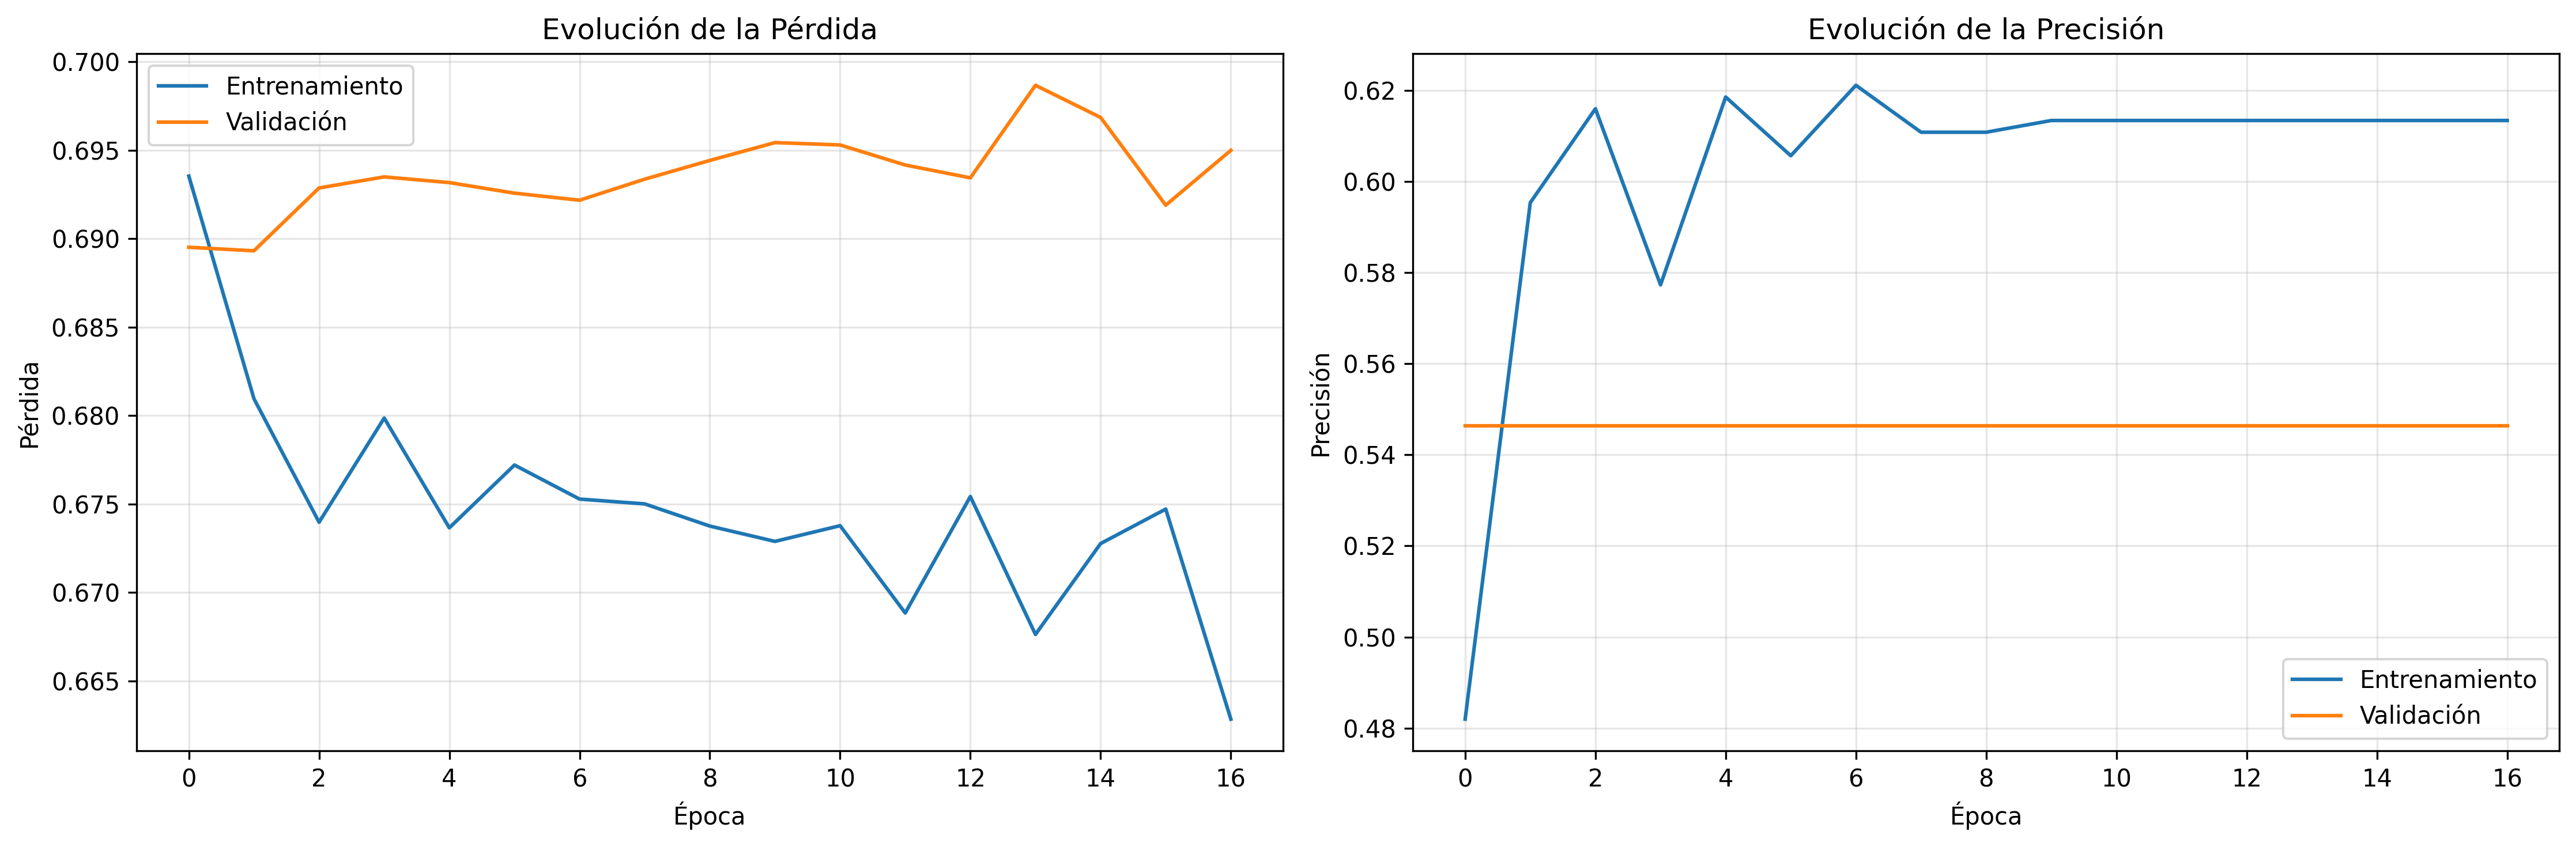
\includegraphics[keepaspectratio]{01-intro.osmnx_files/figure-beamer/cell-7-output-2.png}}

\begin{verbatim}

📊 EVALUACIÓN DEL MODELO LSTM
==================================================
Precisión: 0.5464
Pérdida: 0.6887
Precisión (metric): 0.5464
Recall: 1.0000

📈 REPORTE DE CLASIFICACIÓN:
               precision    recall  f1-score   support

No Inundación       0.00      0.00      0.00        44
   Inundación       0.55      1.00      0.71        53

     accuracy                           0.55        97
    macro avg       0.27      0.50      0.35        97
 weighted avg       0.30      0.55      0.39        97


🎯 MATRIZ DE CONFUSIÓN:
\end{verbatim}

\pandocbounded{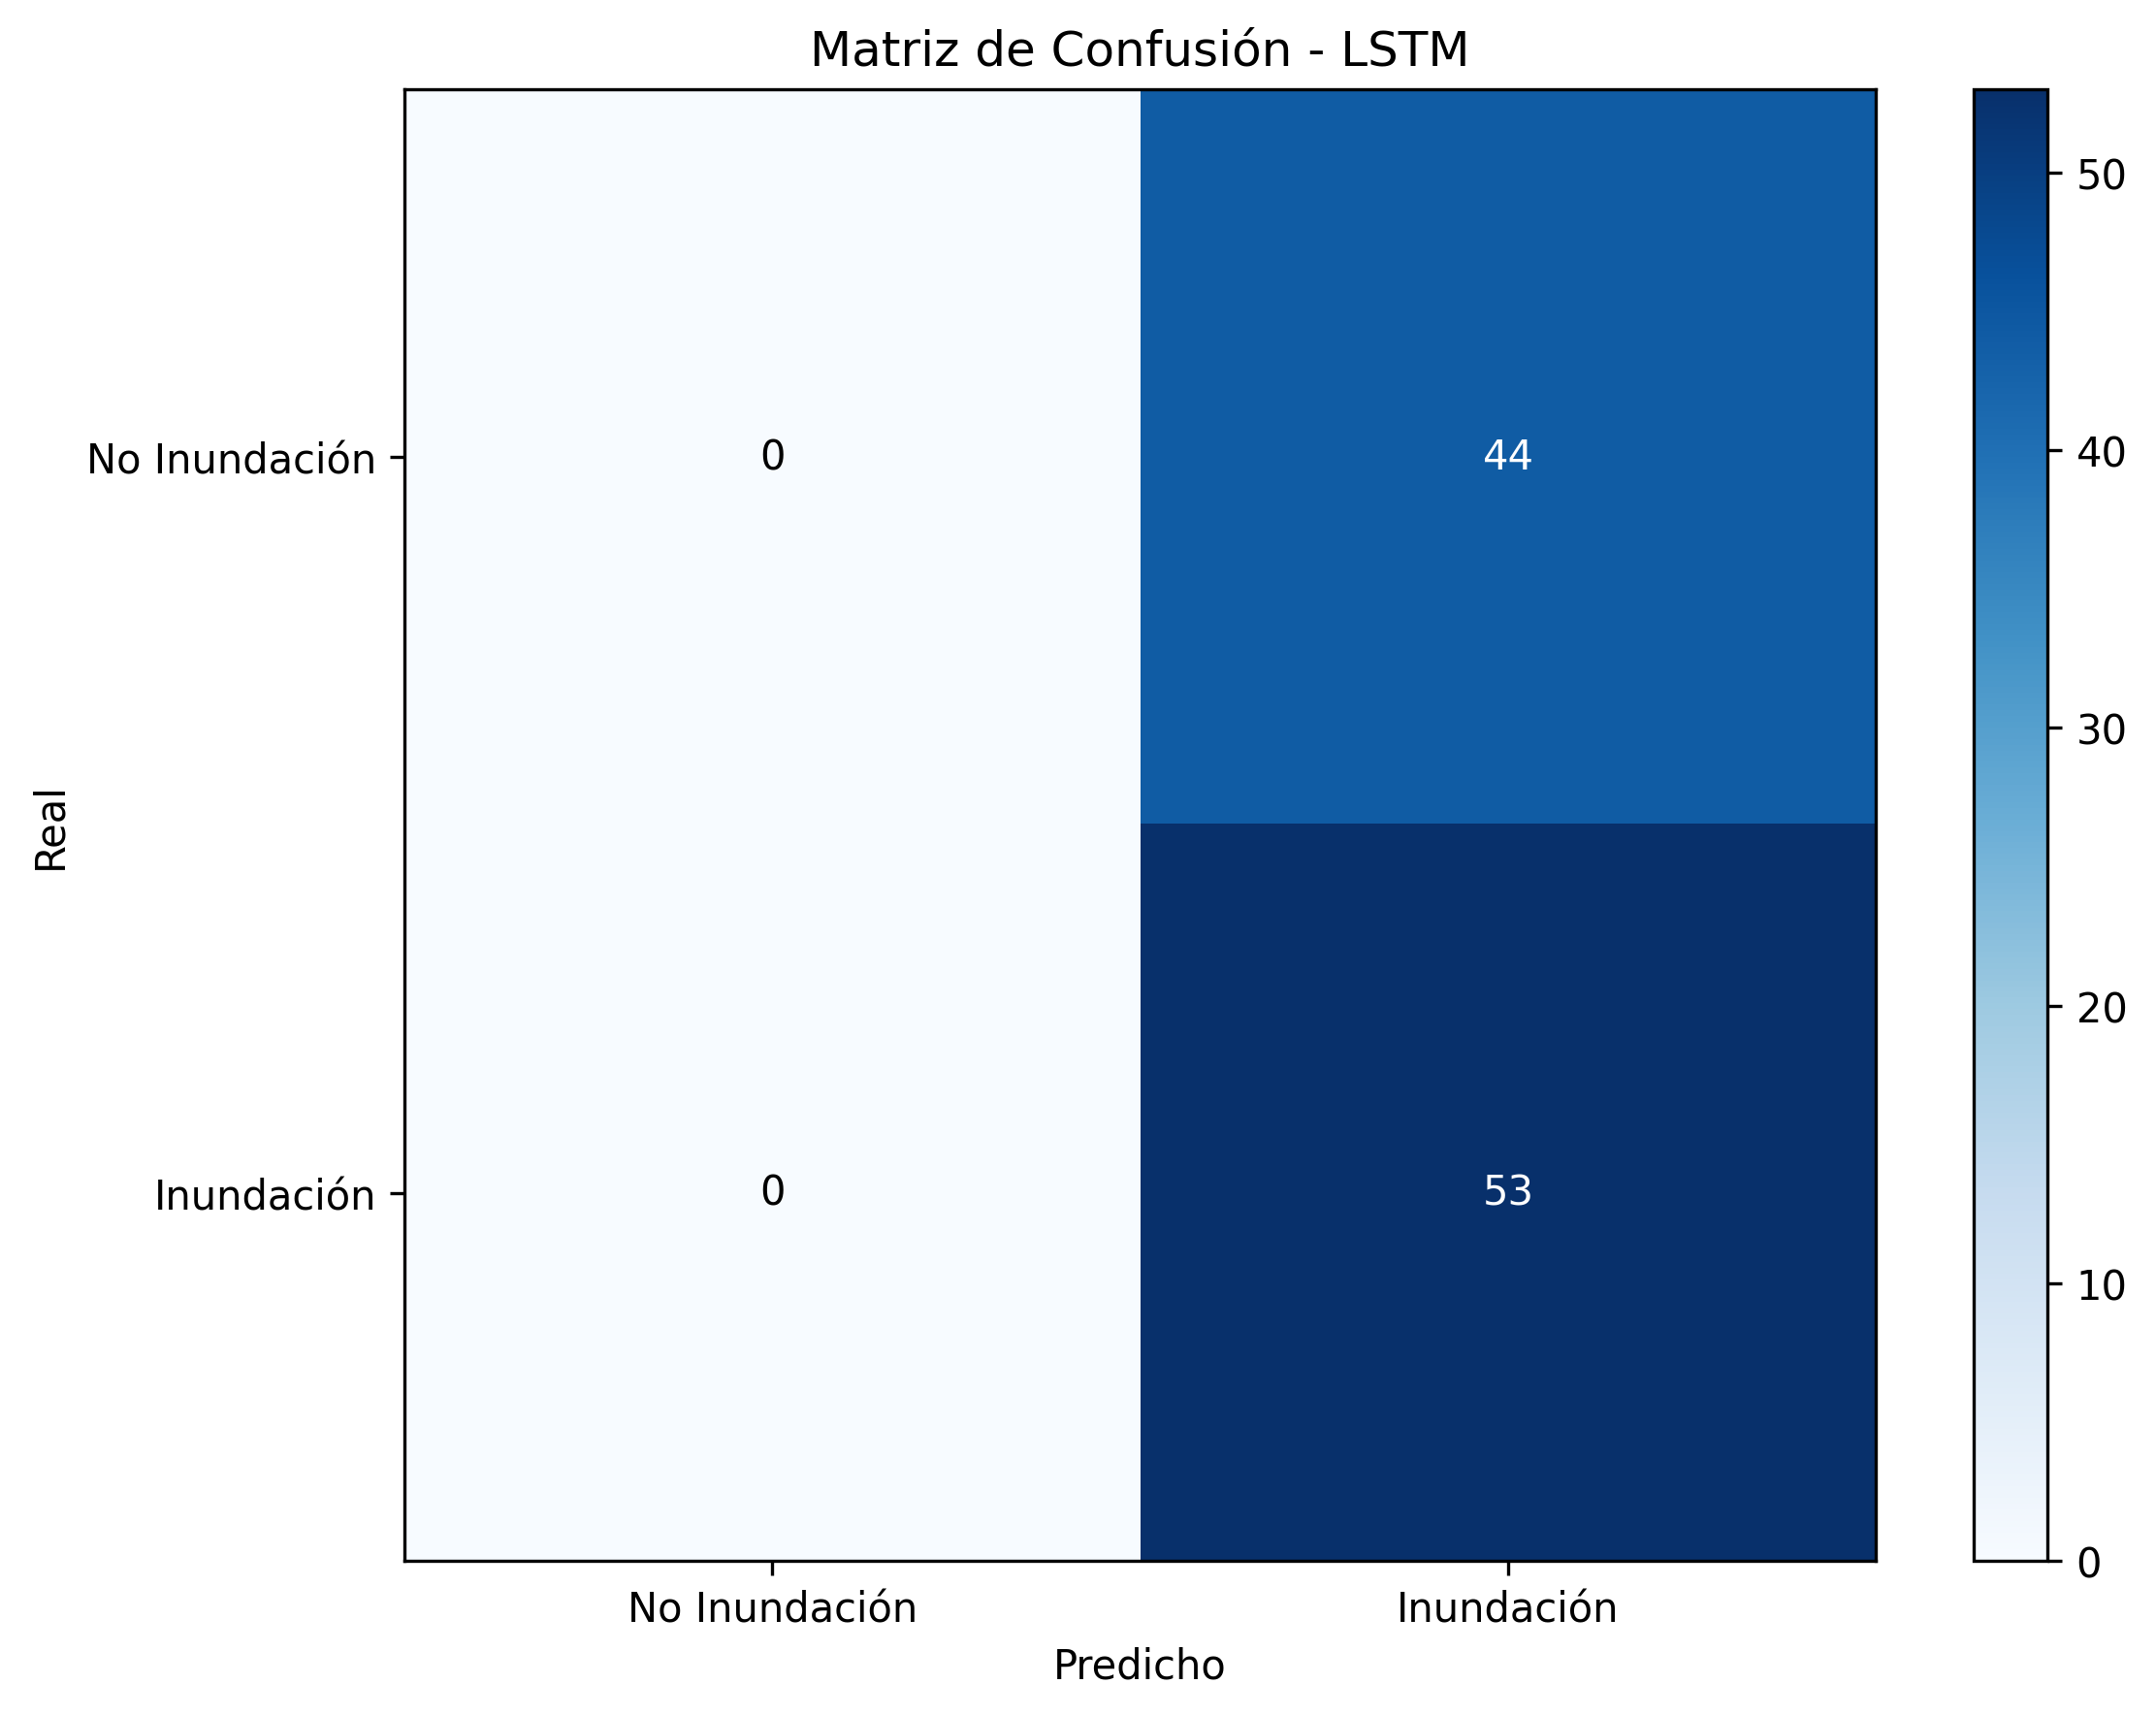
\includegraphics[keepaspectratio]{01-intro.osmnx_files/figure-beamer/cell-7-output-4.png}}

\begin{verbatim}
📊 DIVISIÓN DE DATOS CORREGIDA:
Entrenamiento: 400 muestras
Prueba: 100 muestras
Características: 5
\end{verbatim}

\begin{verbatim}
🏗️ ARQUITECTURA DEL MODELO DENSE:
\end{verbatim}

\begin{verbatim}
Model: "sequential_1"
\end{verbatim}

\begin{verbatim}
┏━━━━━━━━━━━━━━━━━━━━━━━━━━━━━━━━━┳━━━━━━━━━━━━━━━━━━━━━━━━┳━━━━━━━━━━━━━━━┓
┃ Layer (type)                    ┃ Output Shape           ┃       Param # ┃
┡━━━━━━━━━━━━━━━━━━━━━━━━━━━━━━━━━╇━━━━━━━━━━━━━━━━━━━━━━━━╇━━━━━━━━━━━━━━━┩
│ dense_3 (Dense)                 │ (None, 32)             │           192 │
├─────────────────────────────────┼────────────────────────┼───────────────┤
│ dropout_3 (Dropout)             │ (None, 32)             │             0 │
├─────────────────────────────────┼────────────────────────┼───────────────┤
│ dense_4 (Dense)                 │ (None, 16)             │           528 │
├─────────────────────────────────┼────────────────────────┼───────────────┤
│ dropout_4 (Dropout)             │ (None, 16)             │             0 │
├─────────────────────────────────┼────────────────────────┼───────────────┤
│ dense_5 (Dense)                 │ (None, 1)              │            17 │
└─────────────────────────────────┴────────────────────────┴───────────────┘
\end{verbatim}

\begin{verbatim}
 Total params: 737 (2.88 KB)
\end{verbatim}

\begin{verbatim}
 Trainable params: 737 (2.88 KB)
\end{verbatim}

\begin{verbatim}
 Non-trainable params: 0 (0.00 B)
\end{verbatim}

\begin{verbatim}
ARQUITECTURA CON DROPOUT INTEGRADO
\end{verbatim}

\pandocbounded{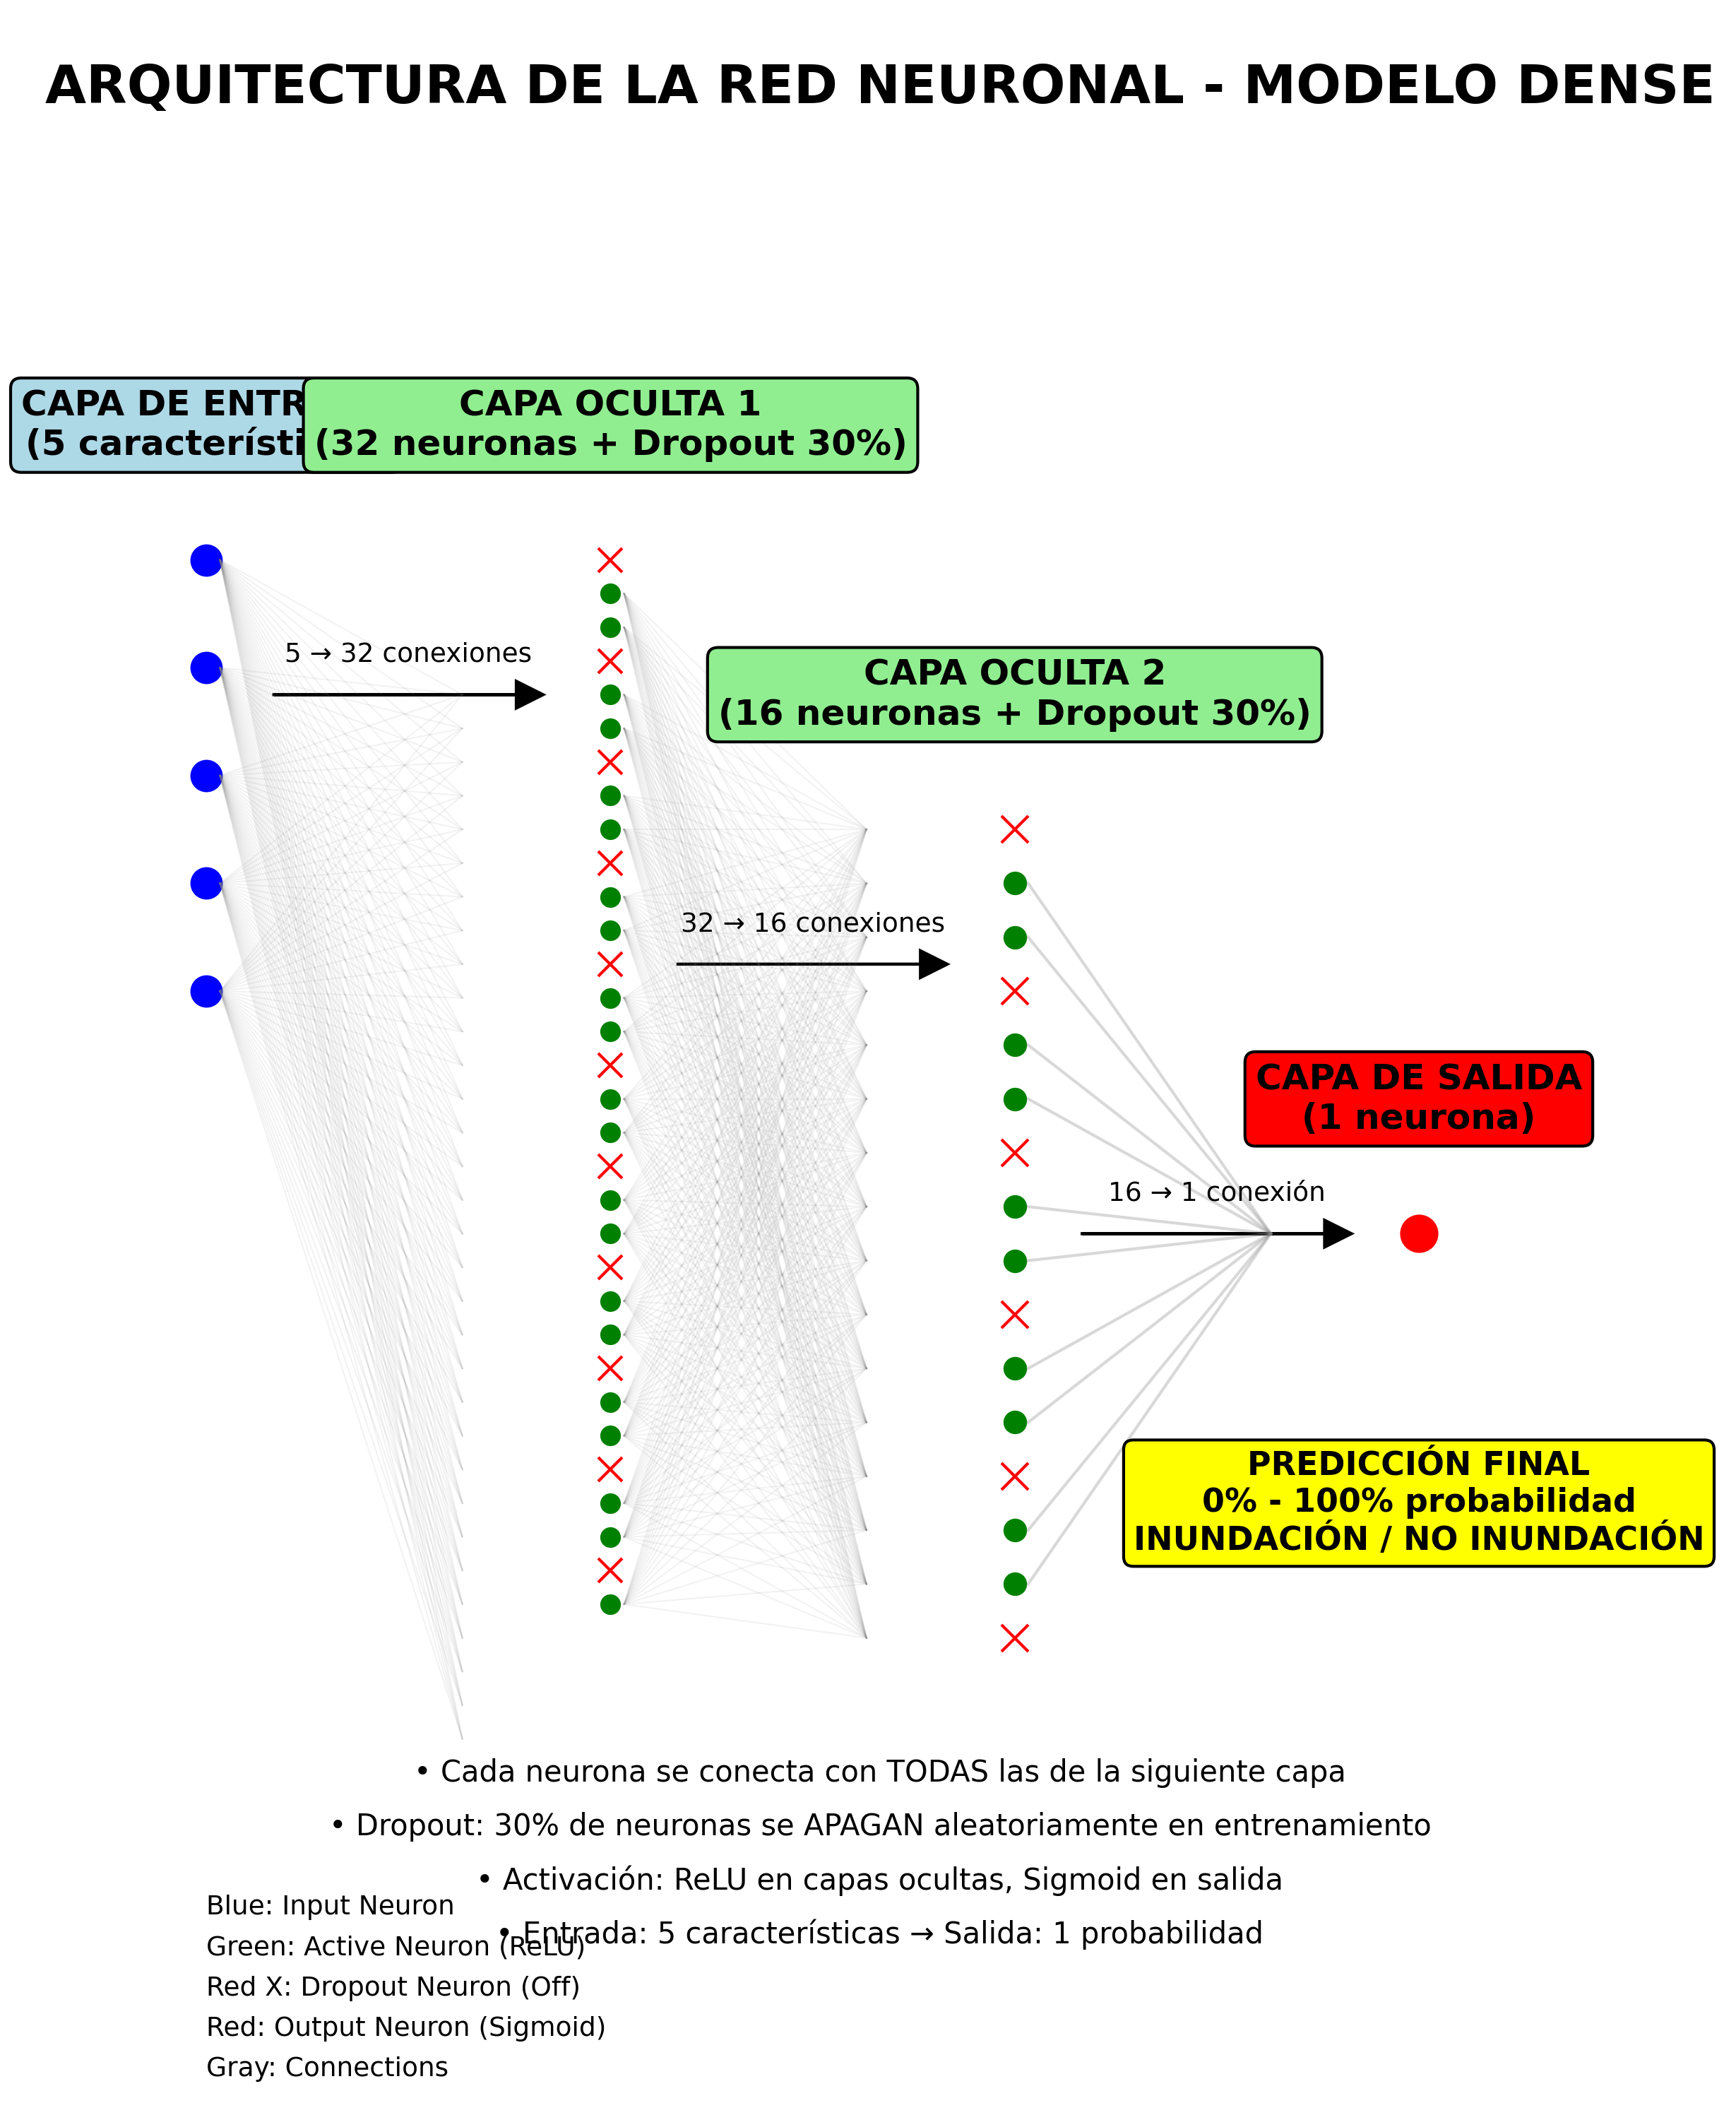
\includegraphics[keepaspectratio]{01-intro.osmnx_files/figure-beamer/cell-10-output-2.png}}

\begin{verbatim}
⚖️ PESOS BALANCEADOS CALCULADOS:
Peso Clase 0 (No inundación): 1.290
Peso Clase 1 (Inundación): 0.816
Epoch 1/50
 1/13 ━━━━━━━━━━━━━━━━━━━━ 20s 2s/step - accuracy: 0.6250 - loss: 0.6871 - precision: 0.8462 - recall: 0.523813/13 ━━━━━━━━━━━━━━━━━━━━ 2s 42ms/step - accuracy: 0.5300 - loss: 0.6909 - precision: 0.6610 - recall: 0.4776 - val_accuracy: 0.6000 - val_loss: 0.6840 - val_precision: 0.6400 - val_recall: 0.5926
Epoch 2/50
 1/13 ━━━━━━━━━━━━━━━━━━━━ 0s 38ms/step - accuracy: 0.4375 - loss: 0.6753 - precision: 0.5882 - recall: 0.476213/13 ━━━━━━━━━━━━━━━━━━━━ 0s 11ms/step - accuracy: 0.5725 - loss: 0.6793 - precision: 0.6637 - recall: 0.6122 - val_accuracy: 0.6300 - val_loss: 0.6741 - val_precision: 0.6545 - val_recall: 0.6667
Epoch 3/50
 1/13 ━━━━━━━━━━━━━━━━━━━━ 0s 41ms/step - accuracy: 0.4375 - loss: 0.6927 - precision: 0.5882 - recall: 0.476213/13 ━━━━━━━━━━━━━━━━━━━━ 0s 11ms/step - accuracy: 0.5950 - loss: 0.6735 - precision: 0.6844 - recall: 0.6286 - val_accuracy: 0.7000 - val_loss: 0.6651 - val_precision: 0.7000 - val_recall: 0.7778
Epoch 4/50
 1/13 ━━━━━━━━━━━━━━━━━━━━ 0s 45ms/step - accuracy: 0.5625 - loss: 0.6567 - precision: 0.7059 - recall: 0.571413/13 ━━━━━━━━━━━━━━━━━━━━ 0s 10ms/step - accuracy: 0.5925 - loss: 0.6755 - precision: 0.6737 - recall: 0.6490 - val_accuracy: 0.7000 - val_loss: 0.6573 - val_precision: 0.7000 - val_recall: 0.7778
Epoch 5/50
 1/13 ━━━━━━━━━━━━━━━━━━━━ 0s 29ms/step - accuracy: 0.6250 - loss: 0.6513 - precision: 0.7143 - recall: 0.714313/13 ━━━━━━━━━━━━━━━━━━━━ 0s 11ms/step - accuracy: 0.6175 - loss: 0.6675 - precision: 0.6811 - recall: 0.7061 - val_accuracy: 0.7100 - val_loss: 0.6493 - val_precision: 0.7049 - val_recall: 0.7963
Epoch 6/50
 1/13 ━━━━━━━━━━━━━━━━━━━━ 0s 39ms/step - accuracy: 0.5312 - loss: 0.6724 - precision: 0.6364 - recall: 0.666713/13 ━━━━━━━━━━━━━━━━━━━━ 0s 11ms/step - accuracy: 0.6375 - loss: 0.6627 - precision: 0.7066 - recall: 0.6980 - val_accuracy: 0.7200 - val_loss: 0.6412 - val_precision: 0.7167 - val_recall: 0.7963
Epoch 7/50
 1/13 ━━━━━━━━━━━━━━━━━━━━ 0s 41ms/step - accuracy: 0.7188 - loss: 0.6360 - precision: 0.7500 - recall: 0.857113/13 ━━━━━━━━━━━━━━━━━━━━ 0s 10ms/step - accuracy: 0.6800 - loss: 0.6523 - precision: 0.7368 - recall: 0.7429 - val_accuracy: 0.7500 - val_loss: 0.6334 - val_precision: 0.7458 - val_recall: 0.8148
Epoch 8/50
 1/13 ━━━━━━━━━━━━━━━━━━━━ 0s 28ms/step - accuracy: 0.7812 - loss: 0.6211 - precision: 0.7917 - recall: 0.904813/13 ━━━━━━━━━━━━━━━━━━━━ 0s 10ms/step - accuracy: 0.6600 - loss: 0.6432 - precision: 0.7243 - recall: 0.7184 - val_accuracy: 0.7600 - val_loss: 0.6244 - val_precision: 0.7586 - val_recall: 0.8148
Epoch 9/50
 1/13 ━━━━━━━━━━━━━━━━━━━━ 0s 43ms/step - accuracy: 0.6562 - loss: 0.6433 - precision: 0.7083 - recall: 0.809513/13 ━━━━━━━━━━━━━━━━━━━━ 0s 12ms/step - accuracy: 0.7075 - loss: 0.6387 - precision: 0.7602 - recall: 0.7633 - val_accuracy: 0.7500 - val_loss: 0.6138 - val_precision: 0.7377 - val_recall: 0.8333
Epoch 10/50
 1/13 ━━━━━━━━━━━━━━━━━━━━ 0s 28ms/step - accuracy: 0.6875 - loss: 0.6179 - precision: 0.7391 - recall: 0.809513/13 ━━━━━━━━━━━━━━━━━━━━ 0s 12ms/step - accuracy: 0.6875 - loss: 0.6382 - precision: 0.7542 - recall: 0.7265 - val_accuracy: 0.7600 - val_loss: 0.6041 - val_precision: 0.7500 - val_recall: 0.8333
Epoch 11/50
 1/13 ━━━━━━━━━━━━━━━━━━━━ 0s 41ms/step - accuracy: 0.6562 - loss: 0.6402 - precision: 0.7273 - recall: 0.761913/13 ━━━━━━━━━━━━━━━━━━━━ 0s 10ms/step - accuracy: 0.6800 - loss: 0.6360 - precision: 0.7577 - recall: 0.7020 - val_accuracy: 0.7800 - val_loss: 0.5950 - val_precision: 0.7759 - val_recall: 0.8333
Epoch 12/50
 1/13 ━━━━━━━━━━━━━━━━━━━━ 0s 36ms/step - accuracy: 0.6562 - loss: 0.6291 - precision: 0.7083 - recall: 0.809513/13 ━━━━━━━━━━━━━━━━━━━━ 0s 13ms/step - accuracy: 0.6475 - loss: 0.6359 - precision: 0.7261 - recall: 0.6816 - val_accuracy: 0.7700 - val_loss: 0.5877 - val_precision: 0.7818 - val_recall: 0.7963
Epoch 13/50
 1/13 ━━━━━━━━━━━━━━━━━━━━ 0s 42ms/step - accuracy: 0.5625 - loss: 0.6388 - precision: 0.6522 - recall: 0.714313/13 ━━━━━━━━━━━━━━━━━━━━ 0s 12ms/step - accuracy: 0.6625 - loss: 0.6217 - precision: 0.7254 - recall: 0.7224 - val_accuracy: 0.7800 - val_loss: 0.5774 - val_precision: 0.7857 - val_recall: 0.8148
Epoch 14/50
 1/13 ━━━━━━━━━━━━━━━━━━━━ 0s 42ms/step - accuracy: 0.6562 - loss: 0.6377 - precision: 0.7273 - recall: 0.761913/13 ━━━━━━━━━━━━━━━━━━━━ 0s 12ms/step - accuracy: 0.6900 - loss: 0.6137 - precision: 0.7410 - recall: 0.7592 - val_accuracy: 0.7800 - val_loss: 0.5676 - val_precision: 0.7759 - val_recall: 0.8333
Epoch 15/50
 1/13 ━━━━━━━━━━━━━━━━━━━━ 0s 24ms/step - accuracy: 0.7188 - loss: 0.6110 - precision: 0.7727 - recall: 0.809513/13 ━━━━━━━━━━━━━━━━━━━━ 0s 8ms/step - accuracy: 0.6825 - loss: 0.6134 - precision: 0.7500 - recall: 0.7224 - val_accuracy: 0.8000 - val_loss: 0.5597 - val_precision: 0.8148 - val_recall: 0.8148
Epoch 16/50
 1/13 ━━━━━━━━━━━━━━━━━━━━ 0s 33ms/step - accuracy: 0.7812 - loss: 0.5758 - precision: 0.8182 - recall: 0.857113/13 ━━━━━━━━━━━━━━━━━━━━ 0s 10ms/step - accuracy: 0.7075 - loss: 0.5860 - precision: 0.7883 - recall: 0.7143 - val_accuracy: 0.8000 - val_loss: 0.5481 - val_precision: 0.8148 - val_recall: 0.8148
Epoch 17/50
 1/13 ━━━━━━━━━━━━━━━━━━━━ 0s 29ms/step - accuracy: 0.7188 - loss: 0.5601 - precision: 0.7727 - recall: 0.809513/13 ━━━━━━━━━━━━━━━━━━━━ 0s 10ms/step - accuracy: 0.7400 - loss: 0.5904 - precision: 0.7950 - recall: 0.7755 - val_accuracy: 0.7900 - val_loss: 0.5364 - val_precision: 0.7895 - val_recall: 0.8333
Epoch 18/50
 1/13 ━━━━━━━━━━━━━━━━━━━━ 0s 43ms/step - accuracy: 0.6250 - loss: 0.6386 - precision: 0.6957 - recall: 0.761913/13 ━━━━━━━━━━━━━━━━━━━━ 0s 12ms/step - accuracy: 0.6900 - loss: 0.5930 - precision: 0.7553 - recall: 0.7306 - val_accuracy: 0.8000 - val_loss: 0.5283 - val_precision: 0.8148 - val_recall: 0.8148
Epoch 19/50
 1/13 ━━━━━━━━━━━━━━━━━━━━ 0s 41ms/step - accuracy: 0.6875 - loss: 0.6012 - precision: 0.7391 - recall: 0.809513/13 ━━━━━━━━━━━━━━━━━━━━ 0s 8ms/step - accuracy: 0.7150 - loss: 0.5846 - precision: 0.7718 - recall: 0.7592 - val_accuracy: 0.8000 - val_loss: 0.5202 - val_precision: 0.8148 - val_recall: 0.8148
Epoch 20/50
 1/13 ━━━━━━━━━━━━━━━━━━━━ 0s 42ms/step - accuracy: 0.6875 - loss: 0.5964 - precision: 0.7619 - recall: 0.761913/13 ━━━━━━━━━━━━━━━━━━━━ 0s 12ms/step - accuracy: 0.7200 - loss: 0.5801 - precision: 0.7806 - recall: 0.7551 - val_accuracy: 0.8000 - val_loss: 0.5115 - val_precision: 0.8148 - val_recall: 0.8148
Epoch 21/50
 1/13 ━━━━━━━━━━━━━━━━━━━━ 0s 44ms/step - accuracy: 0.6875 - loss: 0.5966 - precision: 0.7391 - recall: 0.809513/13 ━━━━━━━━━━━━━━━━━━━━ 0s 12ms/step - accuracy: 0.7000 - loss: 0.5923 - precision: 0.7706 - recall: 0.7265 - val_accuracy: 0.8000 - val_loss: 0.5073 - val_precision: 0.8269 - val_recall: 0.7963
Epoch 22/50
 1/13 ━━━━━━━━━━━━━━━━━━━━ 0s 26ms/step - accuracy: 0.7188 - loss: 0.5405 - precision: 0.7727 - recall: 0.809513/13 ━━━━━━━━━━━━━━━━━━━━ 0s 12ms/step - accuracy: 0.7100 - loss: 0.5721 - precision: 0.7792 - recall: 0.7347 - val_accuracy: 0.8000 - val_loss: 0.4999 - val_precision: 0.8269 - val_recall: 0.7963
Epoch 23/50
 1/13 ━━━━━━━━━━━━━━━━━━━━ 0s 45ms/step - accuracy: 0.7500 - loss: 0.5870 - precision: 0.7826 - recall: 0.857113/13 ━━━━━━━━━━━━━━━━━━━━ 0s 13ms/step - accuracy: 0.6975 - loss: 0.5818 - precision: 0.7870 - recall: 0.6939 - val_accuracy: 0.8000 - val_loss: 0.4923 - val_precision: 0.8269 - val_recall: 0.7963
Epoch 24/50
 1/13 ━━━━━━━━━━━━━━━━━━━━ 0s 46ms/step - accuracy: 0.8438 - loss: 0.5003 - precision: 0.8636 - recall: 0.904813/13 ━━━━━━━━━━━━━━━━━━━━ 0s 13ms/step - accuracy: 0.7250 - loss: 0.5576 - precision: 0.8000 - recall: 0.7347 - val_accuracy: 0.8000 - val_loss: 0.4865 - val_precision: 0.8269 - val_recall: 0.7963
Epoch 25/50
 1/13 ━━━━━━━━━━━━━━━━━━━━ 0s 39ms/step - accuracy: 0.7500 - loss: 0.5274 - precision: 0.7826 - recall: 0.857113/13 ━━━━━━━━━━━━━━━━━━━━ 0s 14ms/step - accuracy: 0.7150 - loss: 0.5657 - precision: 0.7991 - recall: 0.7143 - val_accuracy: 0.8000 - val_loss: 0.4788 - val_precision: 0.8269 - val_recall: 0.7963
Epoch 26/50
 1/13 ━━━━━━━━━━━━━━━━━━━━ 0s 39ms/step - accuracy: 0.7500 - loss: 0.5419 - precision: 0.7600 - recall: 0.904813/13 ━━━━━━━━━━━━━━━━━━━━ 0s 11ms/step - accuracy: 0.7150 - loss: 0.5678 - precision: 0.7860 - recall: 0.7347 - val_accuracy: 0.8000 - val_loss: 0.4738 - val_precision: 0.8269 - val_recall: 0.7963
Epoch 27/50
 1/13 ━━━━━━━━━━━━━━━━━━━━ 0s 43ms/step - accuracy: 0.6875 - loss: 0.5292 - precision: 0.7619 - recall: 0.761913/13 ━━━━━━━━━━━━━━━━━━━━ 0s 11ms/step - accuracy: 0.7025 - loss: 0.5757 - precision: 0.7763 - recall: 0.7224 - val_accuracy: 0.8000 - val_loss: 0.4699 - val_precision: 0.8269 - val_recall: 0.7963
Epoch 28/50
 1/13 ━━━━━━━━━━━━━━━━━━━━ 0s 27ms/step - accuracy: 0.7500 - loss: 0.5773 - precision: 0.8421 - recall: 0.761913/13 ━━━━━━━━━━━━━━━━━━━━ 0s 11ms/step - accuracy: 0.7175 - loss: 0.5687 - precision: 0.8056 - recall: 0.7102 - val_accuracy: 0.8100 - val_loss: 0.4673 - val_precision: 0.8571 - val_recall: 0.7778
Epoch 29/50
 1/13 ━━━━━━━━━━━━━━━━━━━━ 0s 39ms/step - accuracy: 0.6562 - loss: 0.5780 - precision: 0.7273 - recall: 0.761913/13 ━━━━━━━━━━━━━━━━━━━━ 0s 10ms/step - accuracy: 0.7275 - loss: 0.5391 - precision: 0.8148 - recall: 0.7184 - val_accuracy: 0.8000 - val_loss: 0.4579 - val_precision: 0.8400 - val_recall: 0.7778
Epoch 30/50
 1/13 ━━━━━━━━━━━━━━━━━━━━ 0s 36ms/step - accuracy: 0.6875 - loss: 0.5352 - precision: 0.7619 - recall: 0.761913/13 ━━━━━━━━━━━━━━━━━━━━ 0s 11ms/step - accuracy: 0.7475 - loss: 0.5296 - precision: 0.8051 - recall: 0.7755 - val_accuracy: 0.8000 - val_loss: 0.4476 - val_precision: 0.8400 - val_recall: 0.7778
Epoch 31/50
 1/13 ━━━━━━━━━━━━━━━━━━━━ 0s 40ms/step - accuracy: 0.8125 - loss: 0.4707 - precision: 0.8571 - recall: 0.857113/13 ━━━━━━━━━━━━━━━━━━━━ 0s 10ms/step - accuracy: 0.7550 - loss: 0.5247 - precision: 0.8155 - recall: 0.7755 - val_accuracy: 0.8100 - val_loss: 0.4392 - val_precision: 0.8431 - val_recall: 0.7963
Epoch 32/50
 1/13 ━━━━━━━━━━━━━━━━━━━━ 0s 39ms/step - accuracy: 0.6875 - loss: 0.5508 - precision: 0.7391 - recall: 0.809513/13 ━━━━━━━━━━━━━━━━━━━━ 0s 11ms/step - accuracy: 0.7175 - loss: 0.5623 - precision: 0.7797 - recall: 0.7510 - val_accuracy: 0.8100 - val_loss: 0.4369 - val_precision: 0.8571 - val_recall: 0.7778
Epoch 33/50
 1/13 ━━━━━━━━━━━━━━━━━━━━ 0s 35ms/step - accuracy: 0.6562 - loss: 0.5050 - precision: 0.7273 - recall: 0.761913/13 ━━━━━━━━━━━━━━━━━━━━ 0s 10ms/step - accuracy: 0.7025 - loss: 0.5311 - precision: 0.7917 - recall: 0.6980 - val_accuracy: 0.8100 - val_loss: 0.4335 - val_precision: 0.8571 - val_recall: 0.7778
Epoch 34/50
 1/13 ━━━━━━━━━━━━━━━━━━━━ 0s 30ms/step - accuracy: 0.7188 - loss: 0.5238 - precision: 0.8000 - recall: 0.761913/13 ━━━━━━━━━━━━━━━━━━━━ 0s 8ms/step - accuracy: 0.7075 - loss: 0.5307 - precision: 0.7759 - recall: 0.7347 - val_accuracy: 0.8100 - val_loss: 0.4277 - val_precision: 0.8571 - val_recall: 0.7778
Epoch 35/50
 1/13 ━━━━━━━━━━━━━━━━━━━━ 0s 34ms/step - accuracy: 0.7500 - loss: 0.5089 - precision: 0.8095 - recall: 0.809513/13 ━━━━━━━━━━━━━━━━━━━━ 0s 11ms/step - accuracy: 0.7150 - loss: 0.5345 - precision: 0.7937 - recall: 0.7224 - val_accuracy: 0.8100 - val_loss: 0.4221 - val_precision: 0.8431 - val_recall: 0.7963
Epoch 36/50
 1/13 ━━━━━━━━━━━━━━━━━━━━ 0s 43ms/step - accuracy: 0.7500 - loss: 0.5280 - precision: 0.7826 - recall: 0.857113/13 ━━━━━━━━━━━━━━━━━━━━ 0s 11ms/step - accuracy: 0.7525 - loss: 0.5290 - precision: 0.7992 - recall: 0.7959 - val_accuracy: 0.8200 - val_loss: 0.4192 - val_precision: 0.8600 - val_recall: 0.7963
Epoch 37/50
 1/13 ━━━━━━━━━━━━━━━━━━━━ 0s 29ms/step - accuracy: 0.6562 - loss: 0.5130 - precision: 0.7273 - recall: 0.761913/13 ━━━━━━━━━━━━━━━━━━━━ 0s 12ms/step - accuracy: 0.7375 - loss: 0.5214 - precision: 0.8043 - recall: 0.7551 - val_accuracy: 0.8100 - val_loss: 0.4204 - val_precision: 0.8723 - val_recall: 0.7593
Epoch 38/50
 1/13 ━━━━━━━━━━━━━━━━━━━━ 0s 34ms/step - accuracy: 0.7812 - loss: 0.5026 - precision: 0.8500 - recall: 0.809513/13 ━━━━━━━━━━━━━━━━━━━━ 0s 9ms/step - accuracy: 0.7650 - loss: 0.5180 - precision: 0.8386 - recall: 0.7633 - val_accuracy: 0.8200 - val_loss: 0.4205 - val_precision: 0.8913 - val_recall: 0.7593
Epoch 39/50
 1/13 ━━━━━━━━━━━━━━━━━━━━ 0s 34ms/step - accuracy: 0.7500 - loss: 0.4426 - precision: 0.7826 - recall: 0.857113/13 ━━━━━━━━━━━━━━━━━━━━ 0s 12ms/step - accuracy: 0.7450 - loss: 0.5094 - precision: 0.8265 - recall: 0.7388 - val_accuracy: 0.8300 - val_loss: 0.4126 - val_precision: 0.8776 - val_recall: 0.7963
Epoch 40/50
 1/13 ━━━━━━━━━━━━━━━━━━━━ 0s 27ms/step - accuracy: 0.5938 - loss: 0.5628 - precision: 0.7000 - recall: 0.666713/13 ━━━━━━━━━━━━━━━━━━━━ 0s 12ms/step - accuracy: 0.7500 - loss: 0.5116 - precision: 0.8059 - recall: 0.7796 - val_accuracy: 0.8200 - val_loss: 0.4107 - val_precision: 0.8750 - val_recall: 0.7778
Epoch 41/50
 1/13 ━━━━━━━━━━━━━━━━━━━━ 0s 42ms/step - accuracy: 0.6562 - loss: 0.5456 - precision: 0.7273 - recall: 0.761913/13 ━━━━━━━━━━━━━━━━━━━━ 0s 9ms/step - accuracy: 0.7075 - loss: 0.5411 - precision: 0.7759 - recall: 0.7347 - val_accuracy: 0.8200 - val_loss: 0.4124 - val_precision: 0.9091 - val_recall: 0.7407
Epoch 42/50
 1/13 ━━━━━━━━━━━━━━━━━━━━ 0s 28ms/step - accuracy: 0.8438 - loss: 0.4283 - precision: 0.8636 - recall: 0.904813/13 ━━━━━━━━━━━━━━━━━━━━ 0s 7ms/step - accuracy: 0.7700 - loss: 0.5015 - precision: 0.8462 - recall: 0.7633 - val_accuracy: 0.8300 - val_loss: 0.4040 - val_precision: 0.8776 - val_recall: 0.7963
Epoch 43/50
 1/13 ━━━━━━━━━━━━━━━━━━━━ 0s 26ms/step - accuracy: 0.8438 - loss: 0.4607 - precision: 0.8636 - recall: 0.904813/13 ━━━━━━━━━━━━━━━━━━━━ 0s 11ms/step - accuracy: 0.7575 - loss: 0.5231 - precision: 0.8162 - recall: 0.7796 - val_accuracy: 0.8300 - val_loss: 0.4017 - val_precision: 0.8776 - val_recall: 0.7963
Epoch 44/50
 1/13 ━━━━━━━━━━━━━━━━━━━━ 0s 39ms/step - accuracy: 0.8125 - loss: 0.4610 - precision: 0.8261 - recall: 0.904813/13 ━━━━━━━━━━━━━━━━━━━━ 0s 10ms/step - accuracy: 0.7200 - loss: 0.5439 - precision: 0.7879 - recall: 0.7429 - val_accuracy: 0.8200 - val_loss: 0.4043 - val_precision: 0.8750 - val_recall: 0.7778
Epoch 45/50
 1/13 ━━━━━━━━━━━━━━━━━━━━ 0s 25ms/step - accuracy: 0.7500 - loss: 0.4984 - precision: 0.7826 - recall: 0.857113/13 ━━━━━━━━━━━━━━━━━━━━ 0s 8ms/step - accuracy: 0.7375 - loss: 0.5126 - precision: 0.8070 - recall: 0.7510 - val_accuracy: 0.8300 - val_loss: 0.4023 - val_precision: 0.8776 - val_recall: 0.7963
Epoch 46/50
 1/13 ━━━━━━━━━━━━━━━━━━━━ 0s 28ms/step - accuracy: 0.8438 - loss: 0.3899 - precision: 0.8333 - recall: 0.9524 9/13 ━━━━━━━━━━━━━━━━━━━━ 0s 6ms/step - accuracy: 0.7767 - loss: 0.4691 - precision: 0.8244 - recall: 0.8165 13/13 ━━━━━━━━━━━━━━━━━━━━ 0s 13ms/step - accuracy: 0.7575 - loss: 0.5109 - precision: 0.8274 - recall: 0.7633 - val_accuracy: 0.8300 - val_loss: 0.4009 - val_precision: 0.8776 - val_recall: 0.7963
Epoch 47/50
 1/13 ━━━━━━━━━━━━━━━━━━━━ 0s 36ms/step - accuracy: 0.7500 - loss: 0.4998 - precision: 0.8095 - recall: 0.809513/13 ━━━━━━━━━━━━━━━━━━━━ 0s 8ms/step - accuracy: 0.7425 - loss: 0.5255 - precision: 0.8170 - recall: 0.7469 - val_accuracy: 0.8300 - val_loss: 0.4028 - val_precision: 0.9111 - val_recall: 0.7593
Epoch 48/50
 1/13 ━━━━━━━━━━━━━━━━━━━━ 0s 27ms/step - accuracy: 0.8125 - loss: 0.4413 - precision: 0.8571 - recall: 0.857113/13 ━━━━━━━━━━━━━━━━━━━━ 0s 10ms/step - accuracy: 0.7550 - loss: 0.5118 - precision: 0.8356 - recall: 0.7469 - val_accuracy: 0.8300 - val_loss: 0.4020 - val_precision: 0.9111 - val_recall: 0.7593
Epoch 49/50
 1/13 ━━━━━━━━━━━━━━━━━━━━ 0s 26ms/step - accuracy: 0.8125 - loss: 0.4435 - precision: 0.8947 - recall: 0.809513/13 ━━━━━━━━━━━━━━━━━━━━ 0s 11ms/step - accuracy: 0.7375 - loss: 0.5085 - precision: 0.8097 - recall: 0.7469 - val_accuracy: 0.8200 - val_loss: 0.3956 - val_precision: 0.8600 - val_recall: 0.7963
Epoch 50/50
 1/13 ━━━━━━━━━━━━━━━━━━━━ 0s 31ms/step - accuracy: 0.8125 - loss: 0.4445 - precision: 0.8261 - recall: 0.904813/13 ━━━━━━━━━━━━━━━━━━━━ 0s 8ms/step - accuracy: 0.7650 - loss: 0.5111 - precision: 0.8268 - recall: 0.7796 - val_accuracy: 0.8300 - val_loss: 0.3973 - val_precision: 0.8776 - val_recall: 0.7963
Restoring model weights from the end of the best epoch: 49.
\end{verbatim}

\pandocbounded{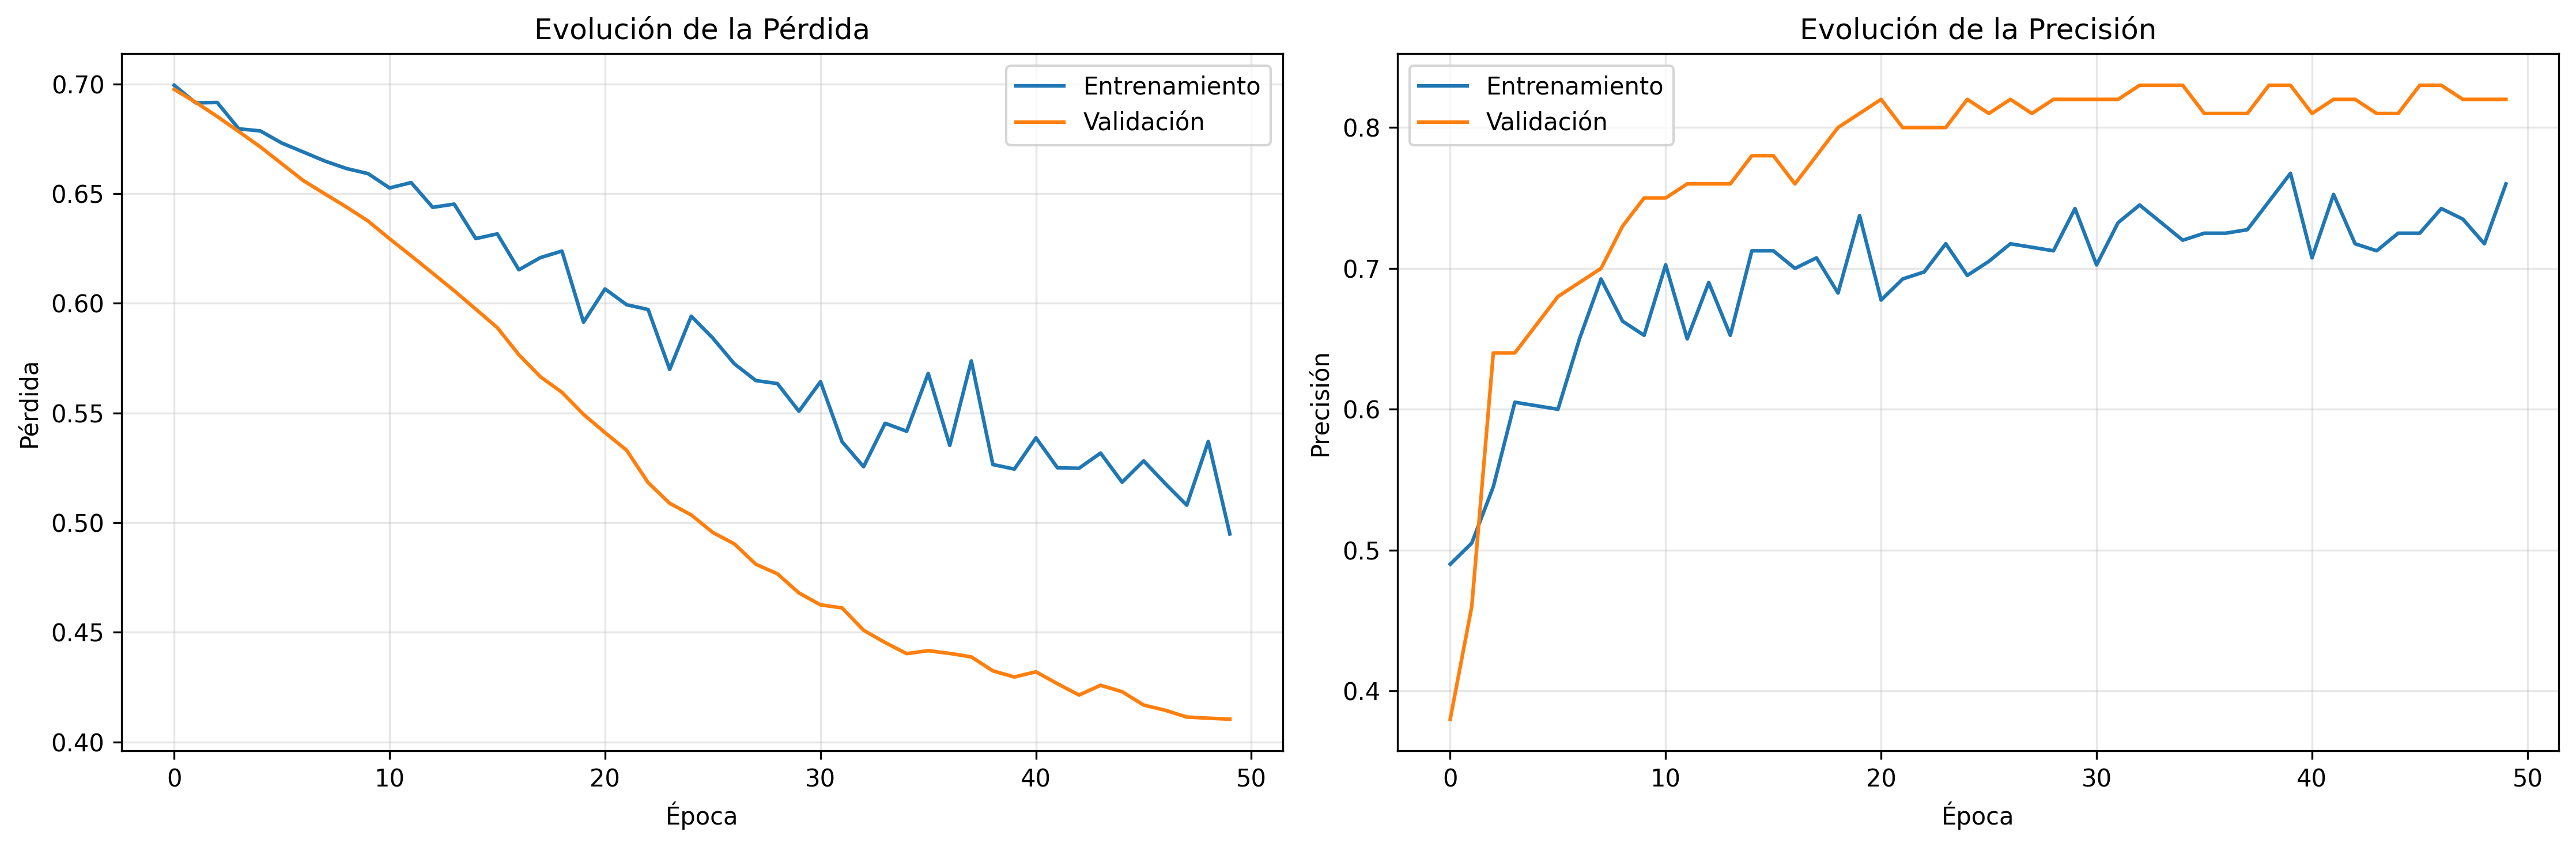
\includegraphics[keepaspectratio]{01-intro.osmnx_files/figure-beamer/cell-11-output-2.png}}

\begin{verbatim}

📊 EVALUACIÓN DEL MODELO DENSE
==================================================
Precisión: 0.8200
Pérdida: 0.3956
Precisión (metric): 0.8600
Recall: 0.7963

📈 REPORTE DE CLASIFICACIÓN:
               precision    recall  f1-score   support

No Inundación       0.78      0.85      0.81        46
   Inundación       0.86      0.80      0.83        54

     accuracy                           0.82       100
    macro avg       0.82      0.82      0.82       100
 weighted avg       0.82      0.82      0.82       100


🎯 MATRIZ DE CONFUSIÓN:
\end{verbatim}

\pandocbounded{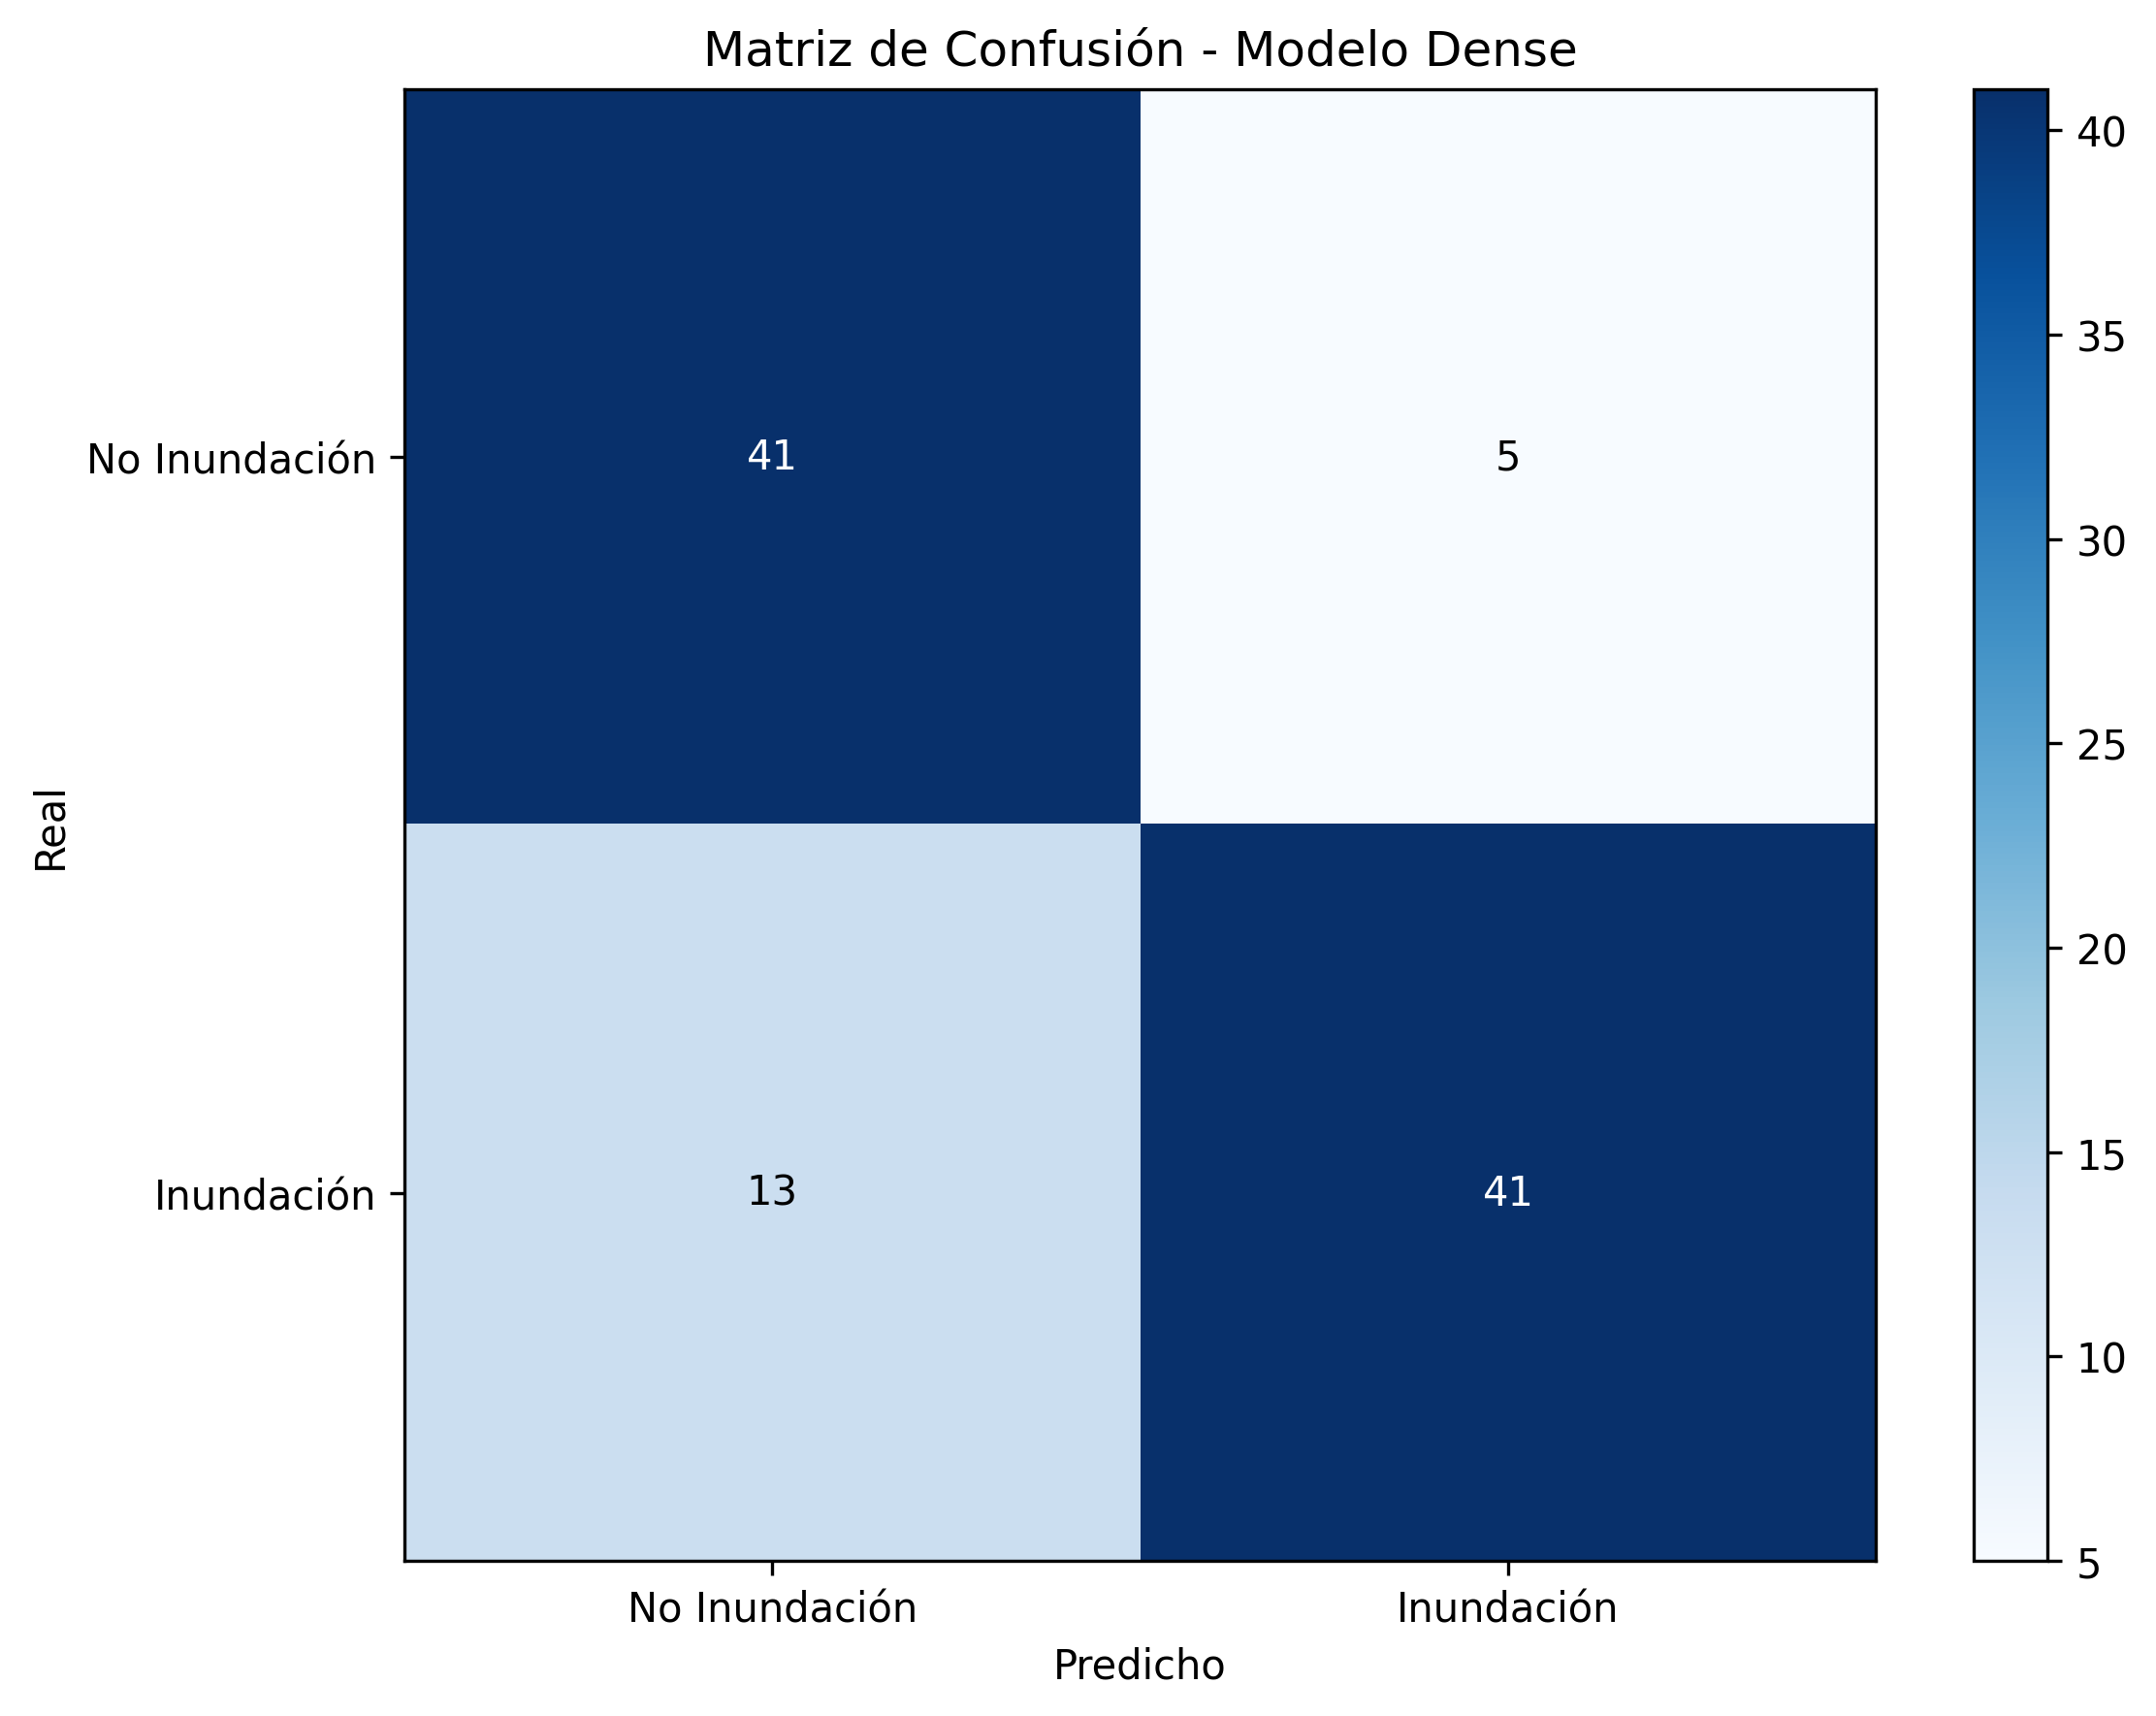
\includegraphics[keepaspectratio]{01-intro.osmnx_files/figure-beamer/cell-11-output-4.png}}
\end{frame}

\begin{frame}{Accuracy}
\phantomsection\label{accuracy}
\begin{block}{Bootstrap}
\phantomsection\label{bootstrap}
Regresión logística = 0.8 Árbol de desición = 0.85 Bagging 30 árboles =
0.83
\end{block}
\end{frame}




\end{document}
